\subsection{Pose Estimation Results}

In these experiments, several current techniques (2D Feature Matching (FM-2D), 3D Feature Matching (FM-3D), ICP and PCA) are compared to the FVR technique in terms of registration accuracy. Comparisons are made over the 3D video frame data described in section \ref{TestDataSection}. As discussed, these 3D video frame scenes contain both different types of environments and are captured using different camera movement techniques. Different camera movements tested include: translational movement, rotational movement and camera zoom. These scenes consist of environments which include: both in-door and out-door environments, low-textured areas and areas which include texture confusion. \\

Experiment results are graphed and presented in this section with the x-axis indicating frame number, whilst the y-axis indicated registration error with respect to the un-registered 3D frames. For example, the $n^{th}$ column along the x-axis represents the error in registering the $n^{th}$ frame with the $(n+1)^{th}$ frame with respect to no registration performed. The y-axis error represents the amount of error (or non-overlap) of the registration between the current and consecutive frames. This error was described in the metrics section (section \ref{metricsSection}). The error function used is the Mean Squared Error $MSE(P,Q)$. This error is computed between the consecutive frames before and after registration. The error post registration is used but is scaled by the prior error, this way all errors are normalized relative to the same value. This error value is computed as in equation \ref{eqn:msesota}. Here, the function $Register(x)$ is replaced by the registration method being tested. \\

\begin{equation} \label{eqn:msesota}
Error(frame_1, frame_2) =  \frac{Register(frame_1), frame2}{MSE(frame_1,frame_2)}
\end{equation}


Each experiment's data is also tabled for convenience. For each algorithm, the average registration error is given. This is computed by summing up the error values for a particular algorithm and dividing by the total number of frames in the experiment. Assisting this is the percent of best results metric. This measures in percentage, the amount of times a particular algorithm achieved the best (lowest error) registration result compared to the other algorithms tested. An algorithm with a lower average error compared to another algorithm would be said to have performed better overall. Additionally, if an algorithm has a higher percentage of best results, it outperformed the other algorithms a majority of the time. If an algorithm achieved the a higher percentage of bests results but a higher average error, this could be explained by outliers. If an algorithm achieved a lower average error but did not achieve the highest percentage of best results, it may be due to having a very competitive and consistent registration error. \\

These experiments were performed by capturing the environment using the ASUS XTION PRO LIVE active depth camera. The frames were captured and stored to a computer hard-drive prior to being processed using each algorithm. \\

%pet0 : apartment texture rotate


\begin{figure}
\centering
\begin{tabular}{ccccccc}
\hline
\textbf{frame} & \textbf{FM-2D} & \textbf{FM-3D} & \textbf{ICP} & \textbf{PCA} & \textbf{FVR} & \textbf{FVR-3D}\\ \hline
1&2&3&4&5&6&7\\
\end{tabular}

\vspace{10mm}
\centering
\begin{tabular}{ccc}
\hline
\textbf{Algorithm} & \textbf{Average Error $\times$ 1000} & \textbf{\% best results}\\ \hline
FM-2D	& 27.52 & ~17.39\\
FM-3D	& 49.80 & 0\\
ICP		& 27.39 & ~17.39\\
PCA		& 37.82 & 0\\
FVR		& 26.87 & ~65.217\\
\end{tabular}

\caption{Statistics for the Apartment Y-Axis Rotation Data Set}
\label{tab:PET0ST}
\end{figure} 

%exxx


\begin{figure}
\centering
\begin{tabular}{ccccccc}
\hline
\textbf{frame} & \textbf{FM-2D} & \textbf{FM-3D} & \textbf{ICP} & \textbf{PCA} & \textbf{FVR} & \textbf{FVR-3D}
\\ \hline
1 & 0.042&0.041&0.037&0.049&0.036&0.141\\
2 & 1.144&1.353&1.526&1.522&1.335&1.227\\
3 & 1.476&0.639&0.527&0.642&0.65&0.524\\
4 & 0.046&0.053&0.053&0.056&0.053&0.061\\
5 & 0.627&0.591&0.622&0.575&0.482&0.631\\
6 & 1.112&1.269&0.844&1.43&1.612&4.108\\
7 & 0.112&0.115&0.069&0.088&0.129&0.089\\
8 & 1.058&1.452&1.122&1.231&1.489&0.773\\
9 & 0.213&0.177&0.172&0.194&0.184&0.153\\
10 & 0.411&0.406&0.426&0.466&0.376&0.356\\
11 & 1.188&1.881&1.146&1.725&1.841&2.447\\
\end{tabular}

\vspace{10mm}
\centering
\begin{tabular}{ccc}
\hline
\textbf{Algorithm} & \textbf{Median Error $\times$ 1000} & \textbf{\% best results}\\ \hline
FM-2D	& 0.627 & ~18.182\%\\
FM-3D	& 0.591 & ~0\%\\
ICP	& 0.527 & ~27.273\%\\
PCA	& 0.575 & ~0\%\\
FVR	& 0.482 & ~18.182\%\\
FVR-3D	& 0.524 & ~36.364\%\\
\end{tabular}

\caption{Statistics for the Apartment Y-Axis Rotation Data Set}
\label{tab:PET0ST}
\end{figure} 


\begin{figure}
\centering
\begin{tabular}{cccccccc}
\hline
\textbf{frame} & \textbf{FM-2D} & \textbf{FM-3D} & \textbf{ICP} & \textbf{PCA} & \textbf{FVR} & \textbf{FFVR} & \textbf{FVR-3D}
\\ \hline
0 & 5.76827 & 5.56533 & 5.2571 & 6.01189 & 6.39835 & 5.58867 & 5.16802\\
1 & 5.99727 & 25864.9 & 5.42174 & 6.48775 & 6.68527 & 6.5874 & 6.36251\\
2 & 5.45112 & 5.66693 & 5.631 & 5.96035 & 6.77246 & 5.49704 & 8.1749\\
3 & 5.59298 & 5.35189 & 4.63077 & 5.30576 & 4.72905 & 6.30678 & 4.76685\\
4 & 4.86083 & 5.80337 & 4.73291 & 5.68578 & 5.98504 & 4.80517 & 5.21404\\
5 & 5.44836 & 9235.71 & 6.36579 & 6.5696 & 6.80482 & 8.37353 & 5.87933\\
6 & 5.23478 & 5.57038 & 6.74113 & 6.07219 & 6.47283 & 6.6327 & 5.2392\\
7 & 7.58893 & 19552.4 & 7.03406 & 7.71283 & 7.08542 & 8.35665 & 7.00138\\
8 & 4.63246 & 4.90545 & 4.65159 & 4.59741 & 5.44854 & 5.04928 & 5.3405\\
9 & 5.39655 & 5.42601 & 5.30633 & 5.8112 & 5.82338 & 5.17521 & 4.85065\\
10 & 5.27262 & 6.47485 & 5.09788 & 5.2152 & 6.40838 & 5.40483 & 5.20236\\
11 & 5.5436 & 3766.04 & 5.461 & 5.69188 & 8.5856 & 5.38372 & 6.0163\\
12 & 4.81508 & 130851 & 4.59424 & 5.62355 & 4.50471 & 5.4209 & 5.06482\\
13 & 4.00779 & 4214.9 & 3.92531 & 4.59796 & 4.30731 & 4.0559 & 4.14147\\
14 & 4.28421 & 5.10618 & 4.52619 & 4.72885 & 4.43962 & 3.98497 & 4.44409\\
15 & 4.48135 & 5.21103 & 4.8585 & 4.81297 & 5.44388 & 4.90852 & 4.56727\\
16 & 6.64 & 6.64684 & 4.59663 & 5.06546 & 6.65699 & 5.21956 & 4.34174\\
17 & 5.13697 & 5.17023 & 4.59618 & 5.1936 & 5.83675 & 5.74173 & 4.53822\\
18 & 4.64986 & 4.93649 & 4.52268 & 4.97689 & 4.70366 & 5.04662 & 4.60245\\
19 & 4.84677 & 6.083 & 5.40279 & 5.32683 & 5.36619 & 5.86823 & 5.96715\\
20 & 5.2719 & 15604 & 5.12423 & 6.43023 & 5.41725 & 5.99697 & 6.22611\\
21 & 4.46766 & 4.85459 & 5.03549 & 5.04746 & 5.14205 & 6.75146 & 4.35163\\
22 & 5.66482 & 99429.5 & 5.5768 & 5.65694 & 7.29495 & 5.95852 & 5.29211\\
23 & 5.92643 & 937.023 & 7.08007 & 6.11491 & 7.55055 & 6.13918 & 5.36414\\
24 & 6.16881 & 6.17455 & 6.07677 & 6.41914 & 5.8878 & 6.42176 & 5.90582\\
25 & 5.17311 & 5.10011 & 4.93152 & 6.16958 & 4.54295 & 5.49422 & 5.68012\\
26 & 5.31275 & 87463.4 & 4.3208 & 5.49572 & 6.3327 & 5.35319 & 4.91221\\
27 & 5.55481 & 5.36219 & 5.11154 & 5.23516 & 5.69667 & 5.64758 & 5.52259\\
28 & 4.38553 & 5.24997 & 4.97161 & 4.72492 & 5.13863 & 12.8416 & 4.26143\\
\end{tabular}
\vspace{10mm}
\centering
\begin{tabular}{ccc}
\hline
\textbf{Algorithm} & \textbf{Median Error $\times$ 1000} & \textbf{\% best results}\\ \hline
FM2D	& 5.27 & 17.24\%\\
FM3D	& 5.8 & 0\%\\
ICP	& 5.1 & 31.03\%\\
PCA	& 5.62 & 3.45\%\\
FVR	& 5.84 & 10.34\%\\
FFVR	& 5.59 & 6.9\%\\
FVR3D	& 5.21 & 31.03\%\\
\end{tabular}
\caption{Statistics for the Kitti Stereo Data Set}
\label{tab:kittistereo}
\end{figure} 




%pet0 : apartment texture rotate
\begin{figure}
\centering
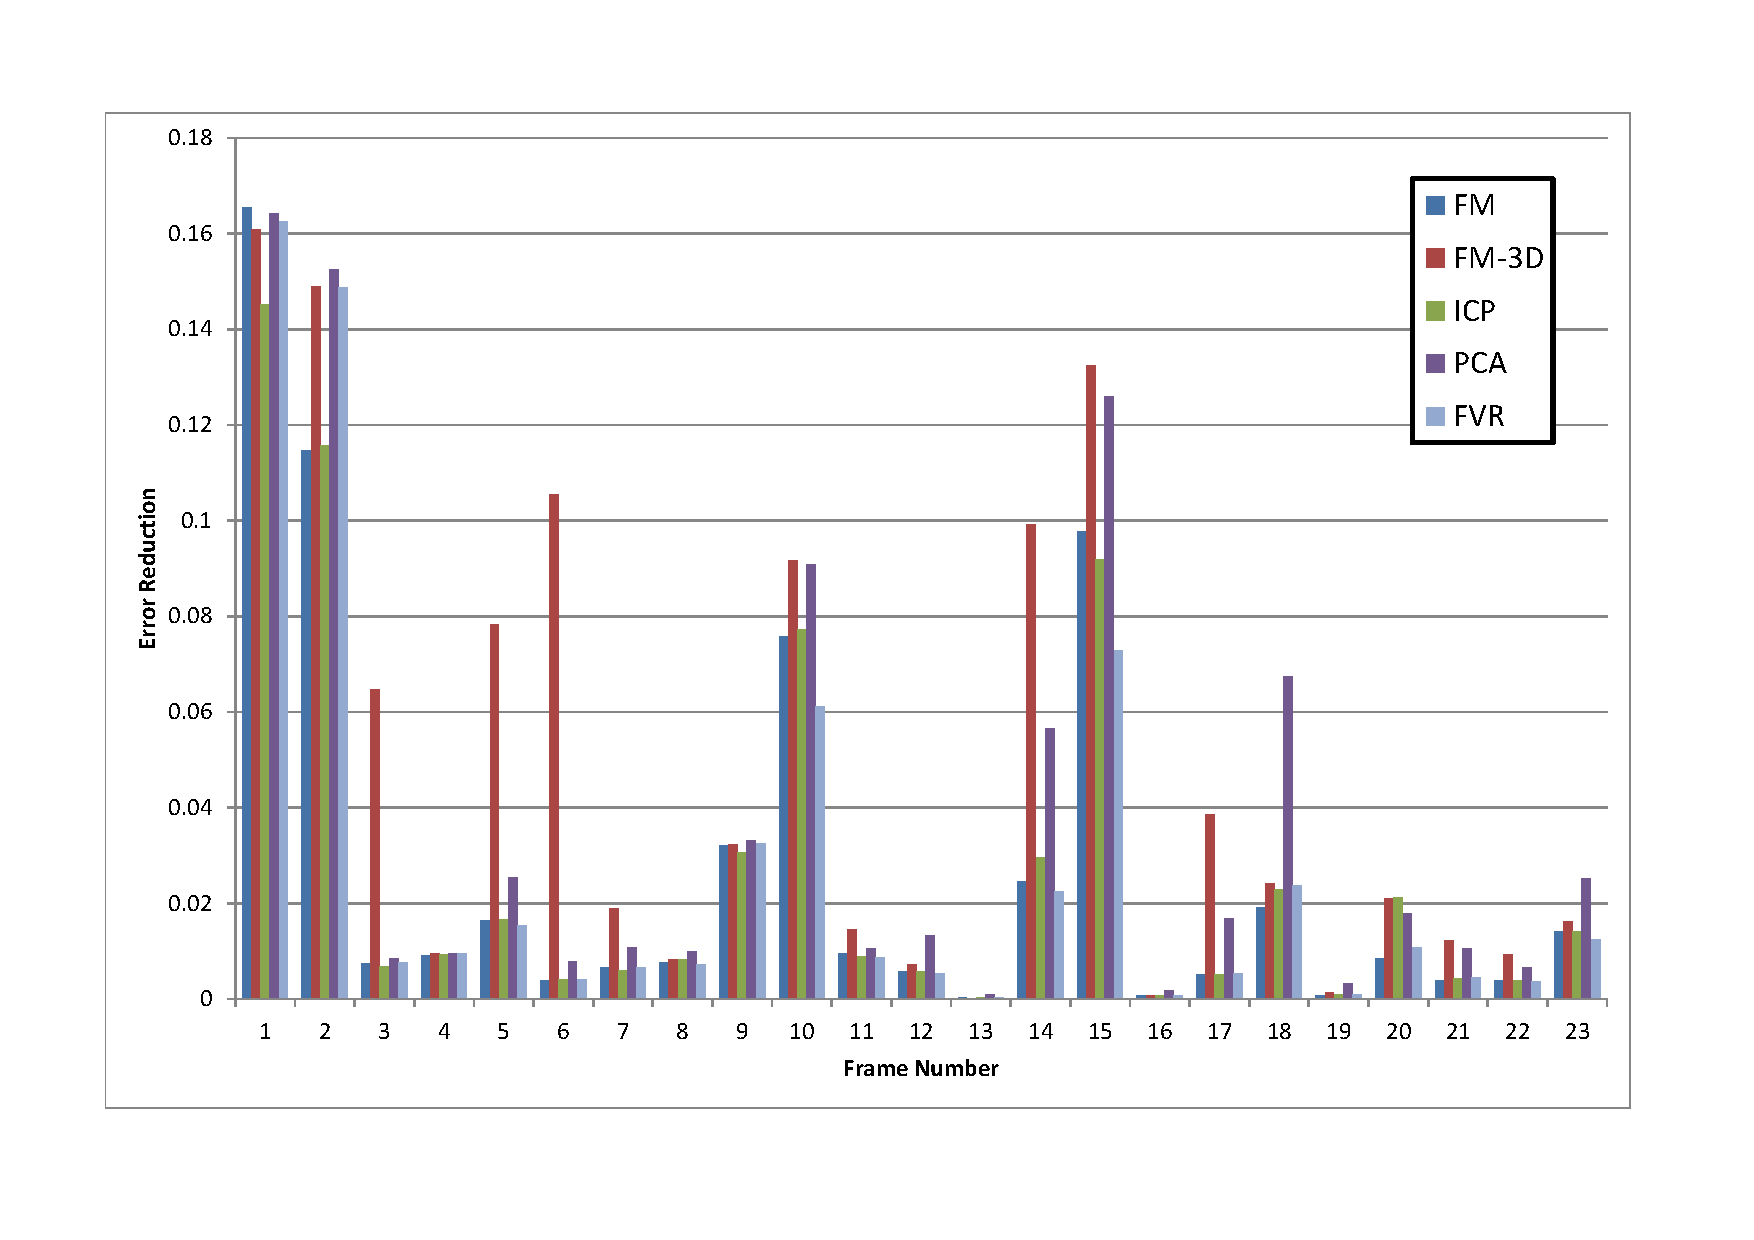
\includegraphics[width=6in]{images/results/Apartment_Texture_Rotate}
\caption{Registration Error for the Apartment Y-Axis Rotation Data Set}
\label{fig:PET0}

\begin{tabular}{ccc}
\hline
\textbf{Algorithm} & \textbf{Average Error $\times$ 1000} & \textbf{\% best results}\\ \hline
FM-2D	& 27.52 & ~17.39\\
FM-3D	& 49.80 & 0\\
ICP		& 27.39 & ~17.39\\
PCA		& 37.82 & 0\\
FVR		& 26.87 & ~65.217\\
\end{tabular}
\captionof{table}{Statistics for the Apartment Y-Axis Rotation Data Set}
%\label{tab:PET0ST}
\end{figure} 



In figure \ref{fig:PET0}, feature-matching, 3D-feature-matching, ICP, PCA and Fourier Volume Registration (FVR) were tested. Overall, the 2D feature matching has the lowest average error out of the two feature matching methods. This scene is of the inside of an apartment which contains various pieces of furniture and plenty of textural information. The camera was rotated about the y-axis whilst moving the camera (translation) across the room. ICP performed slightly better than FM-2D but the FVR algorithm was shown to have the lowest average error. Additionally to being consistent, the FVR method had the largest percentage of best results. At a value of ~65\%, this means that for around 65\% of the frames, the FVR method gave the optimal result compared to the others. Here ICP and FM-2D performed similarly. Both PCA and FM-3D performed worse-off. In this type of scene where much texture information is plentiful, this is ideal for feature matching methods. Additionally, frames were not highly separated so it is ideal for ICP also. ICP is shown to be consistent yet does not reach the performance of the FVR algorithm. \\


%pet 1 apartment texture rotate x-axis
\begin{figure}
\centering
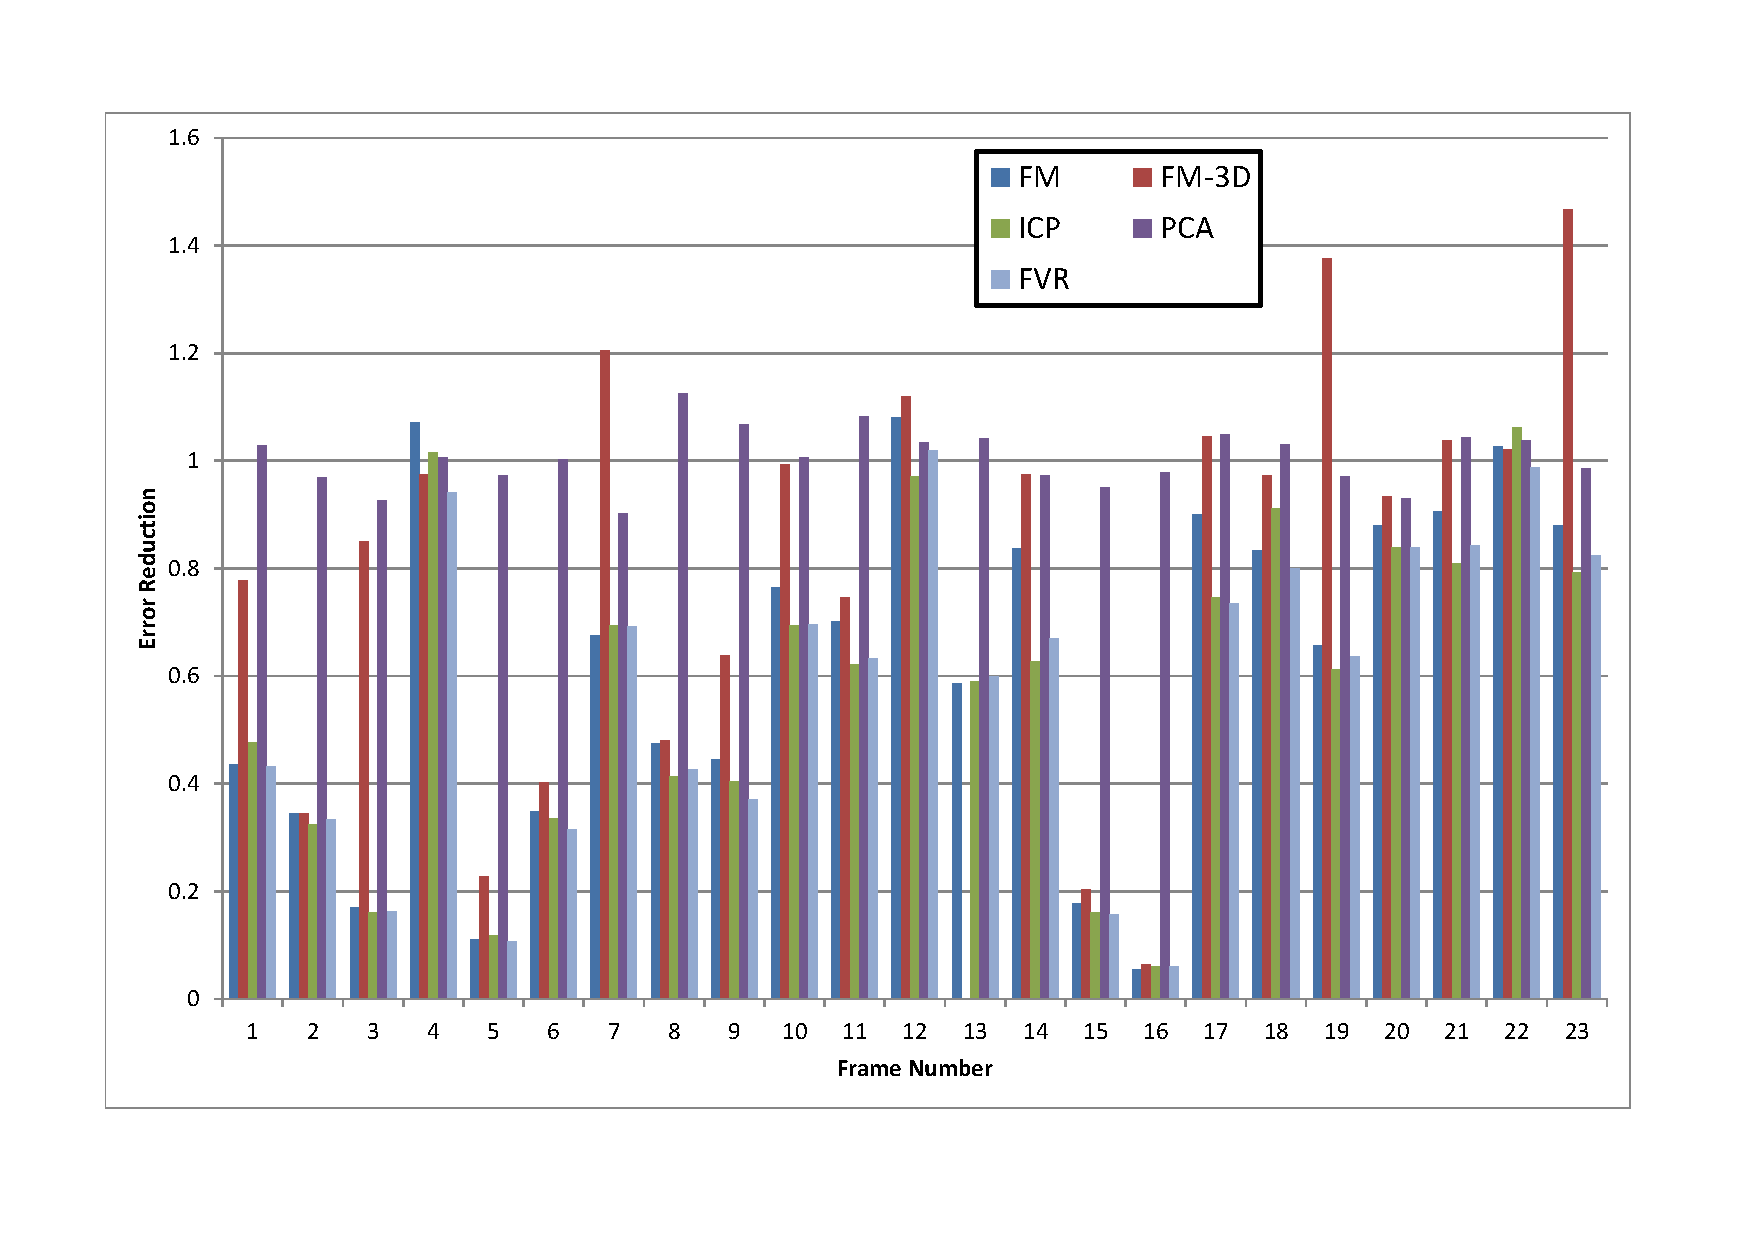
\includegraphics[width=6in]{images/results/Apartment_Texture_Rotate_XAxis}
\caption{Registration Error for the Apartment X/Y-Axis Rotation Data Set}
\label{fig:PET1}

\begin{tabular}{ccc}
\hline
\textbf{Algorithm} & \textbf{Average Error $\times$ 1000} & \textbf{\% best result}\\ \hline
FM-2D	& 624.3 & ~13.04\\
FM-3D	& 841.3 & 0\\
ICP		& 584.2 & ~43.48\\
PCA		& 1005.1 & 0\\
FVR		& 576.86 & ~43.48\\
\end{tabular}
\captionof{table}{Statistics for the Apartment X/Y-Axis Rotation Data Set}
%\label{tab:PET1ST}
\end{figure} 



Figure \ref{fig:PET1} shows registration errors for the the apartment scene again, this time the camera is moved about the x-axis predominantly, again this scene contains lots of texture. In a about 43\% of the frames, FVR either outperforms the other algorithms. Here, ICP performs next best with the same statistic for the percentage of best result metric. 2D-feature matching is also very competitive with 3D-feature-matching and PCA failing to register most frames as accurately as the others. In the case of PCA, when there is not enough overlapping data to register, inaccurate registrations occur. When the FVR technique uses PCA, it only uses the primary axis, and refines the alignment in the secondary stage. Additionally, according to the average error metric, the FVR is shown to be the best performer with the lowest average error. \\


%pet 2 Boxes Y-Axis Rotation Data Set
\begin{figure}
\centering
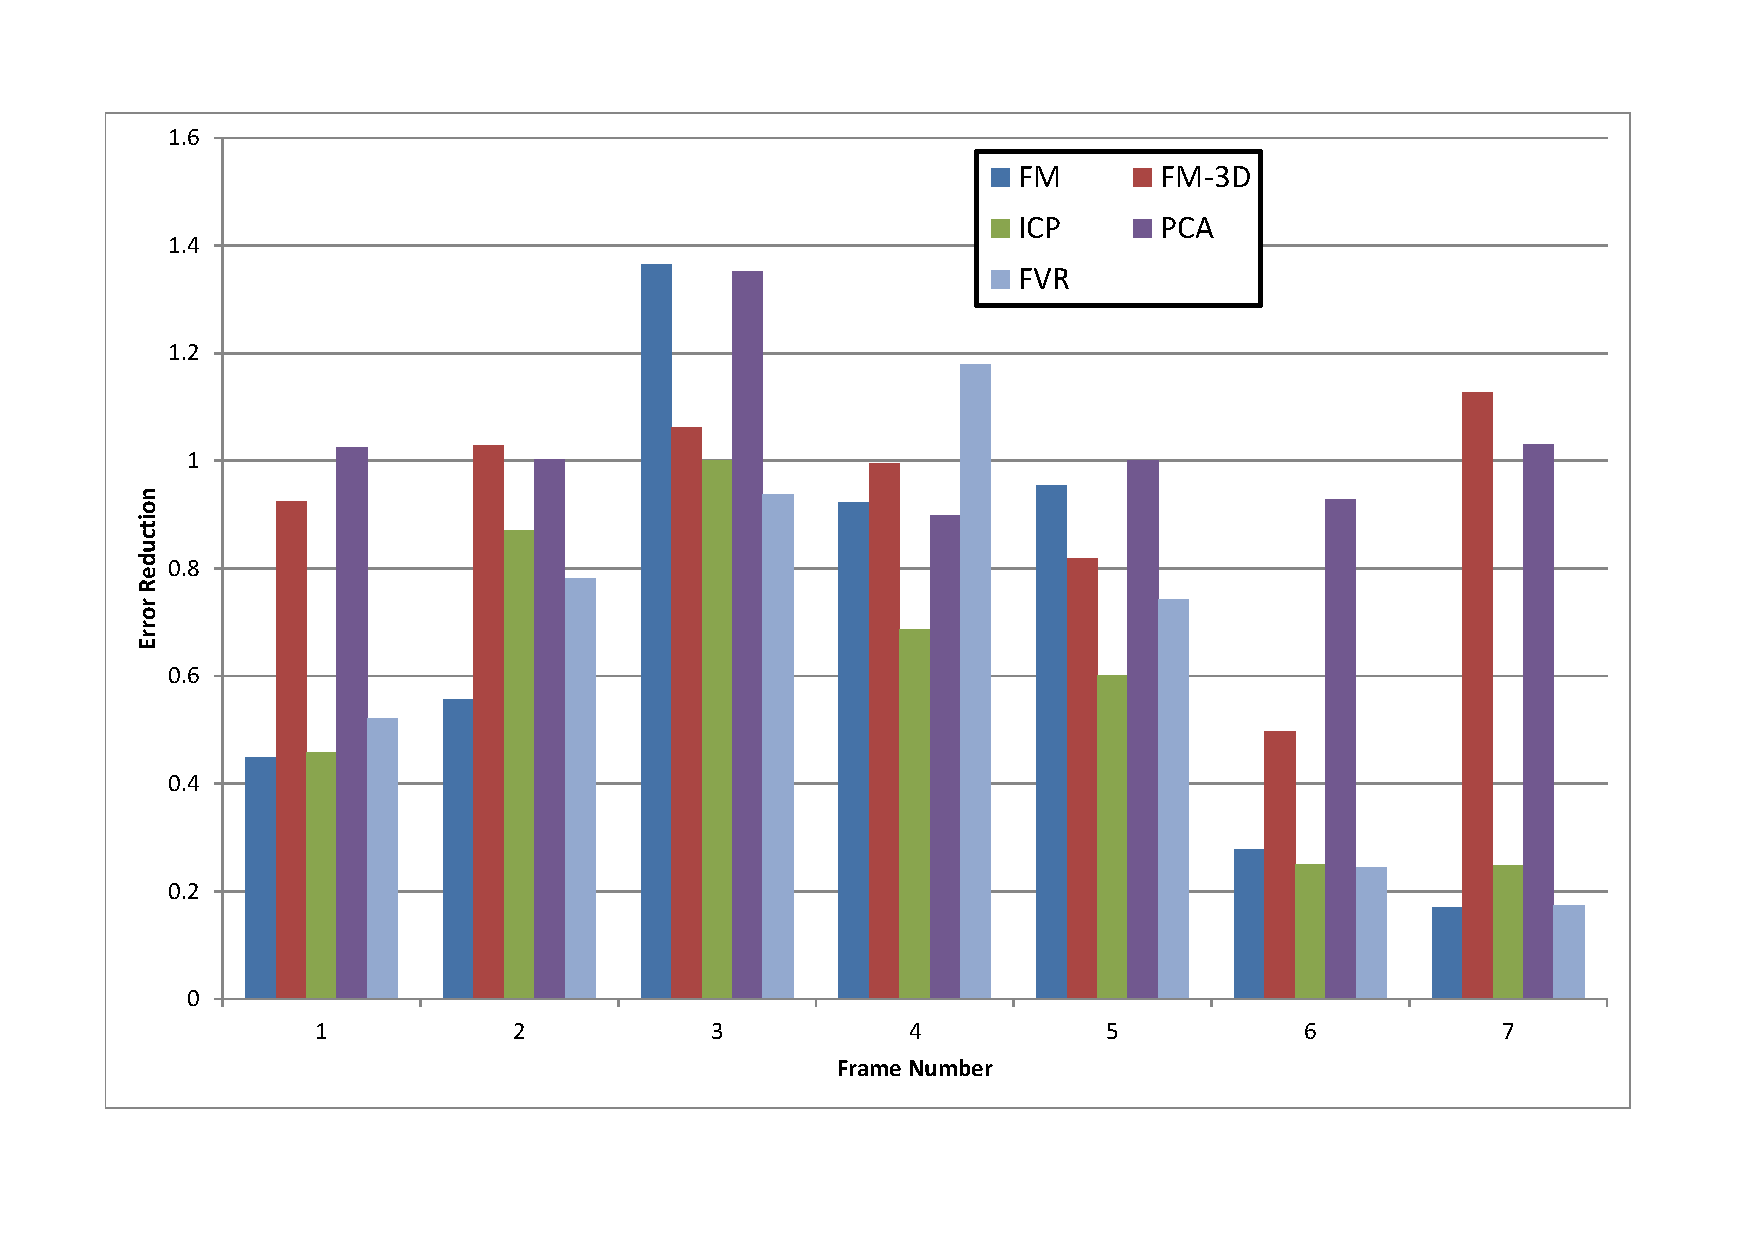
\includegraphics[width=6in]{images/results/Boxes_Texture_Rotate}
\caption{Registration Error for the Boxes Y-Axis Rotation Data Set}
\label{fig:PET2}

\begin{tabular}{ccc}
\hline
\textbf{Algorithm} & \textbf{Average Error $\times$ 1000} & \textbf{\% best result}\\ \hline
FM-2D	& 574.48 & ~33.3\\
FM-3D	& 19502.3 & ~3.7\\
ICP		& 550.3 & ~33.3\\
PCA		& 981.6 & 0\\
FVR		& 508.13 & ~29.6\\
\end{tabular}
\captionof{table}{Statistics for the Boxes Y-Axis Rotation Data Set}
%\label{tab:PET2ST}
\end{figure} 





In figure \ref{fig:PET2} 7 frame registration errors are shown for the Boxes scene. This scene contains camera rotation about the y-axis where in different views were observed during frame capture. In around 30\% of the frames, FVR outperformed the other algorithms. Here both IPC and FM-2D performed similarly. Despite not achieving the largest number of optimal results, the FVR has the lowest average error, meaning it consistently outperformed others or at least matched their performance closely.  \\



%pet 3 Boxes Zoom Data Set
\begin{figure}
\centering
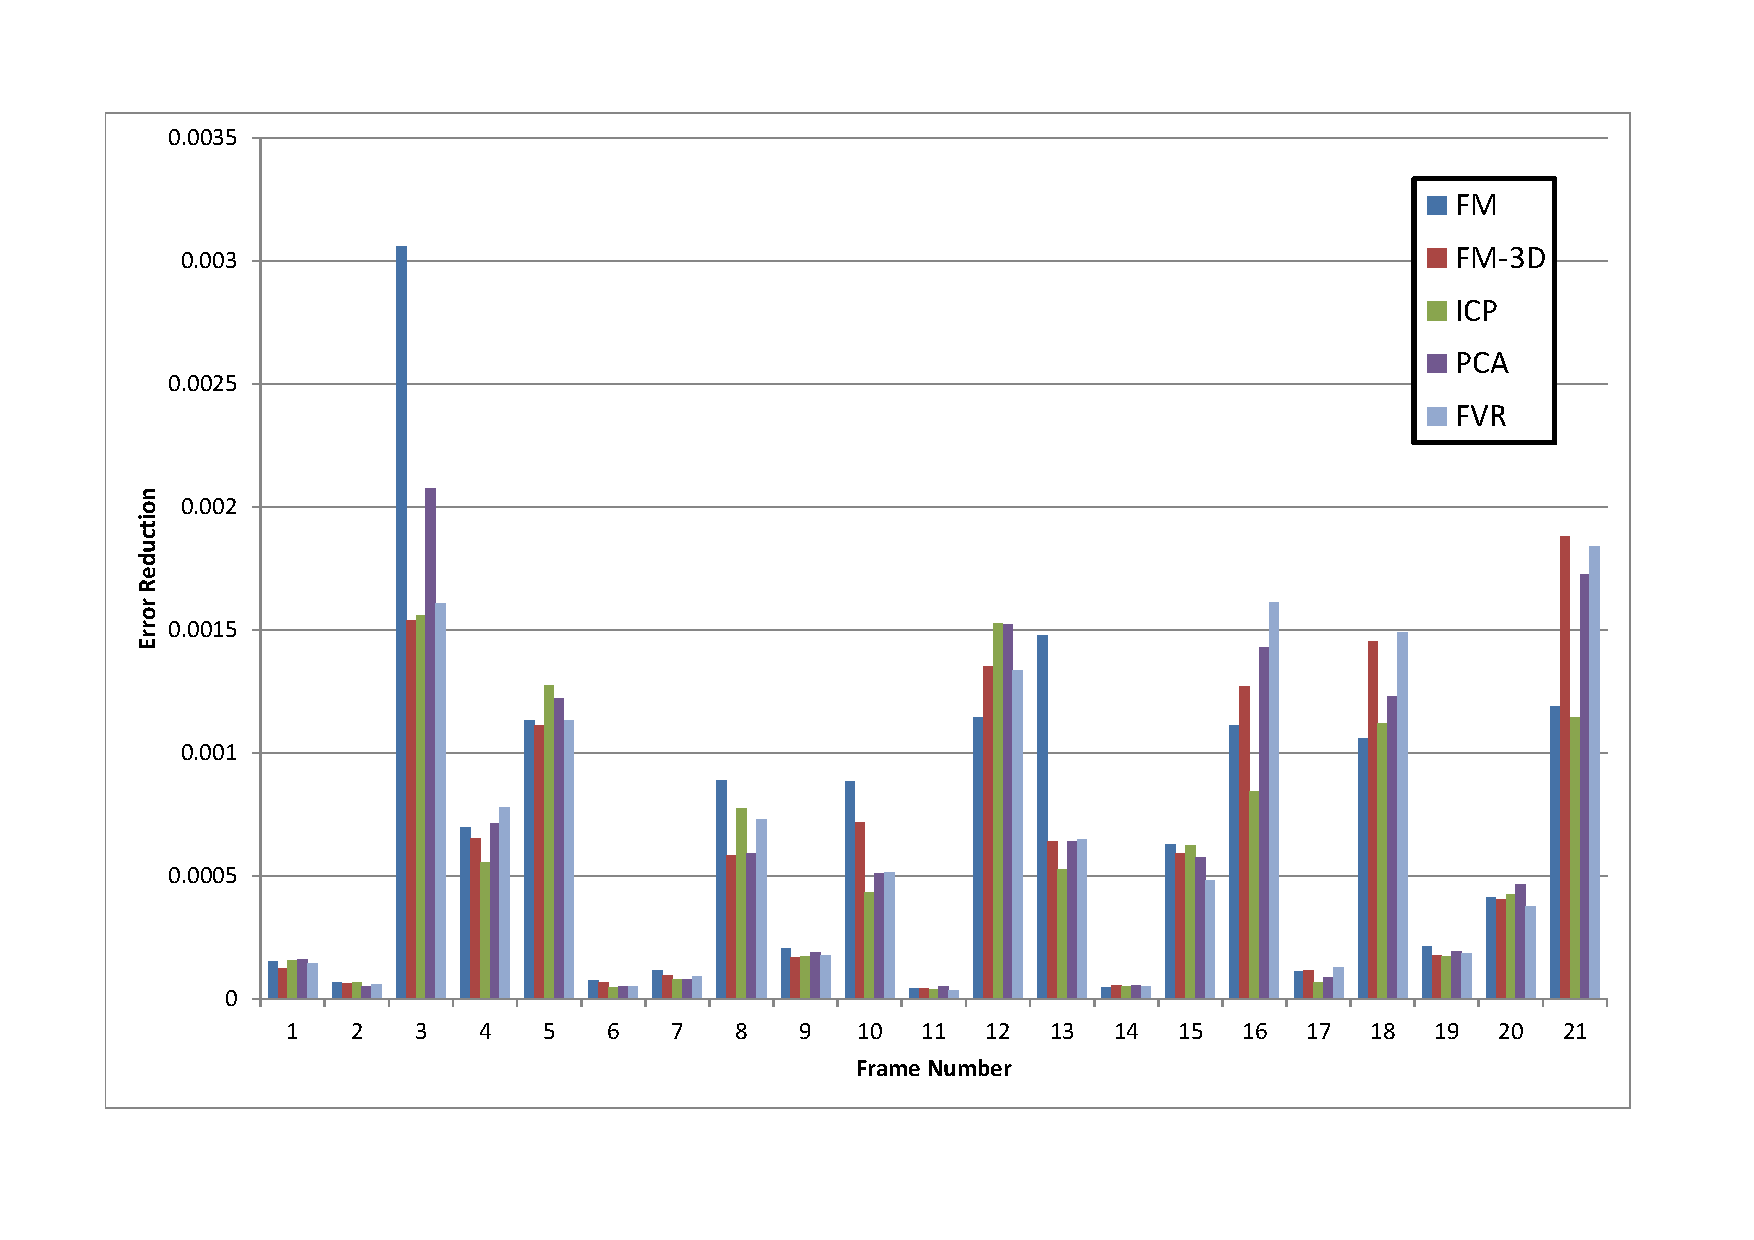
\includegraphics[width=6in]{images/results/Boxes_Texture_ZoomOut}
\caption{Registration Error for the Boxes Zoom Data Set}
\label{fig:PET3}

\begin{tabular}{ccc}
\hline
\textbf{Algorithm} & \textbf{Average Error $\times$ 1000} & \textbf{\% best result}\\ \hline
FM-2D	& 0.68 & ~18.18\\
FM-3D	& 0.73 & 0\\
ICP		& 0.59 & ~27.27\\
PCA		& 0.73 & 0\\
FVR		& 0.65 & ~54.54\\
\end{tabular}
\captionof{table}{Statistics for the Boxes Zoom Data Set}
%\label{tab:PET3ST}
\end{figure} 

%pet 4 Boxes Zoom Data Set
\begin{figure}
\centering
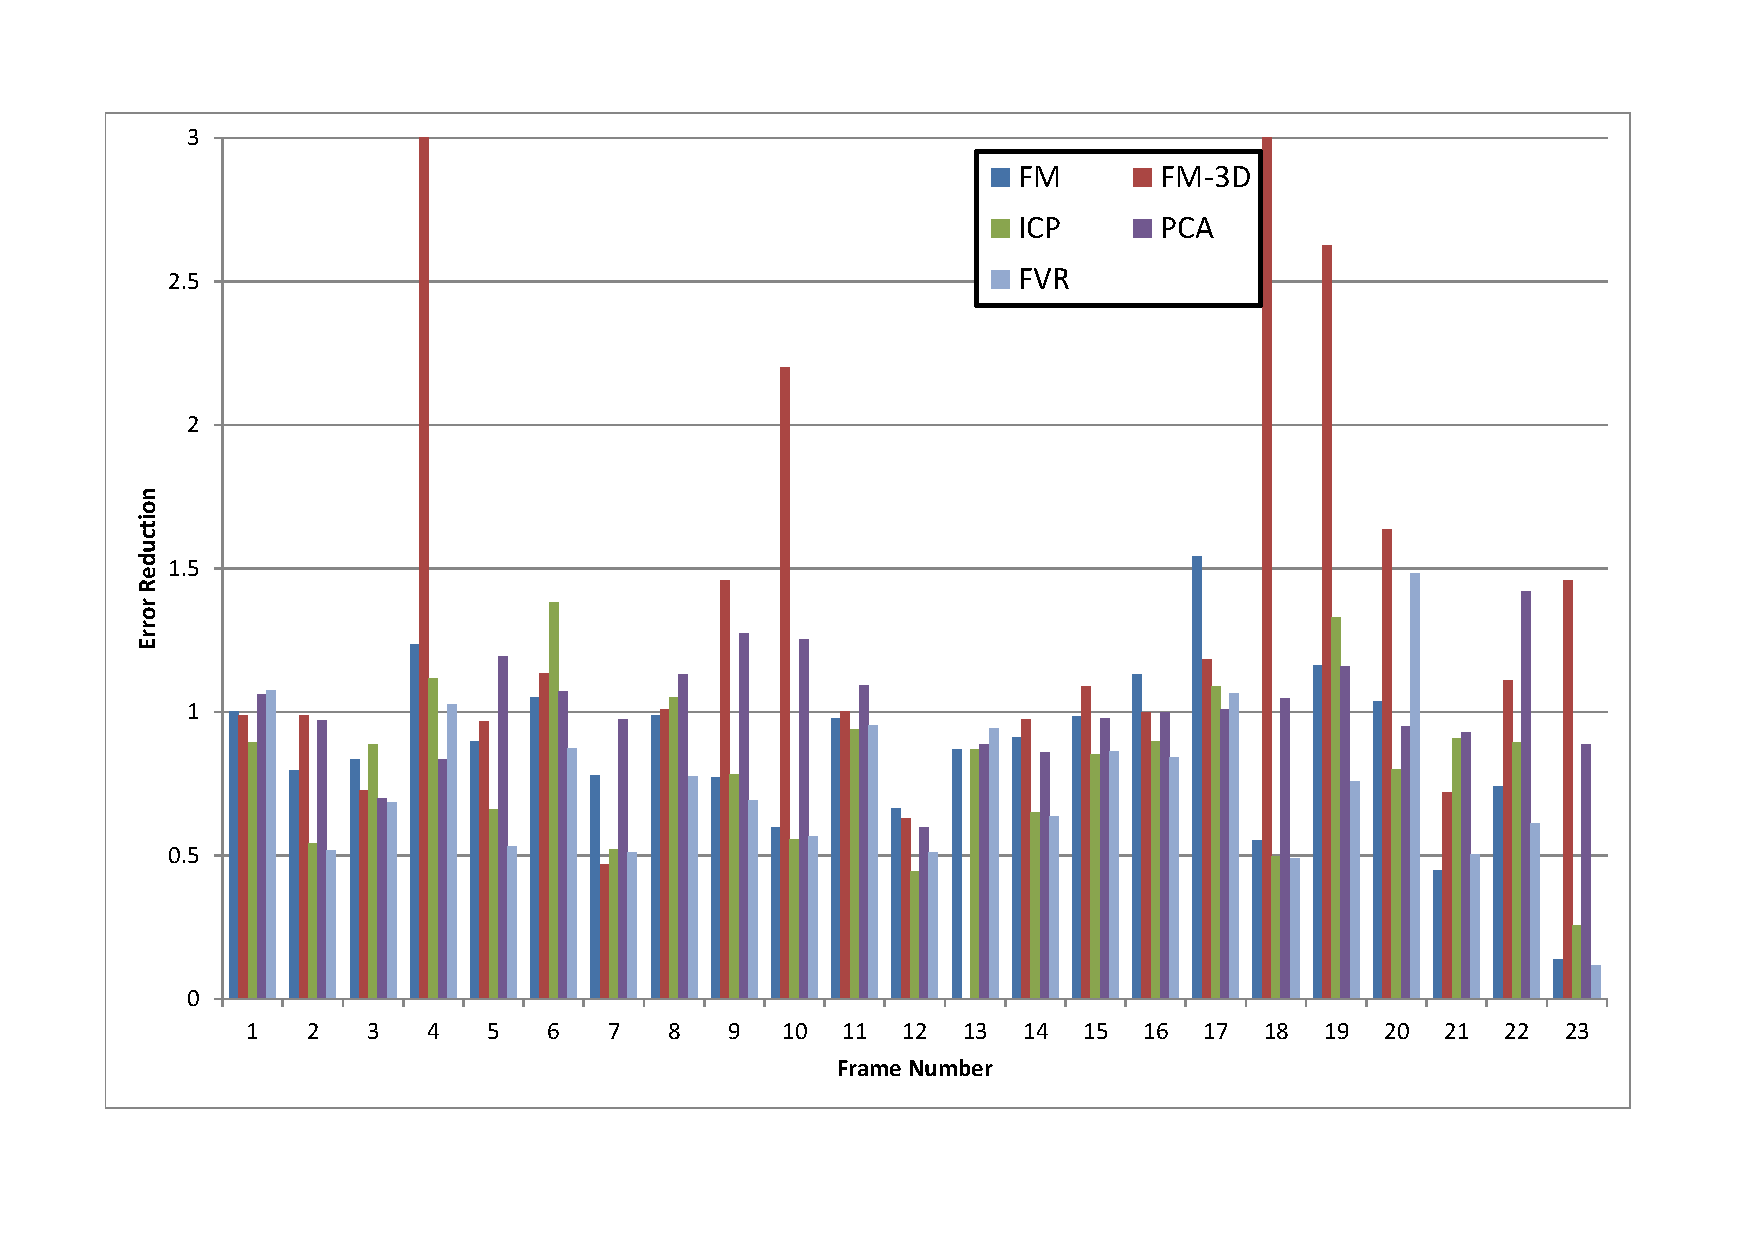
\includegraphics[width=6in]{images/results/Desk_Texture_Translation}
\caption{Registration Error for the Desk Translation Data Set}
\label{fig:PET4}

\begin{tabular}{ccc}
\hline
\textbf{Algorithm} & \textbf{Average Error $\times$ 1000} & \textbf{\% best result}\\ \hline
FM-2D	& 874.18 & ~8.7\\
FM-3D	& 1447.42 & ~4.35\\
ICP		& 818.41 & ~26.09\\
PCA		& 1011.59 & ~8.7\\
FVR		& 740.33 & ~52.17\\
\end{tabular}
\captionof{table}{Statistics for the Desk Translation Data Set}
%\label{tab:PET4ST}
\end{figure} 


Experiment results for another boxes scene are shown in figure \ref{fig:PET3}. In this scene, the camera was moved forward and backward, effectively changing focus on different parts of the same set of boxes at different times during frame capture. Here the FVR algorithm achieved the optimal result in around 55\% of the frames. ICP performed next best with a percentage of best results of around 27\%. Additionally the FVR method also achieved a lower average error compared to the other algorithms. \\


In ~52\% of the frames of the desk translation data-set in figure \ref{fig:PET4}, the FVR method outperformed others relative to just ~26\% for ICP, ~9\% for 2D-feature-matching and PCA and ~4\% for 3D-feature-matching. This data-set tests each procedure's ability to reconstruct a scene captured by moving a camera forward along a path. 3D feature matching was a notable poor performer here. Additionally FVR outperformed the other methods overall in terms of having the lowest average error. \\

%pet 5 Texture Confusion Indoor-Space Translation Data Set
\begin{figure}
\centering
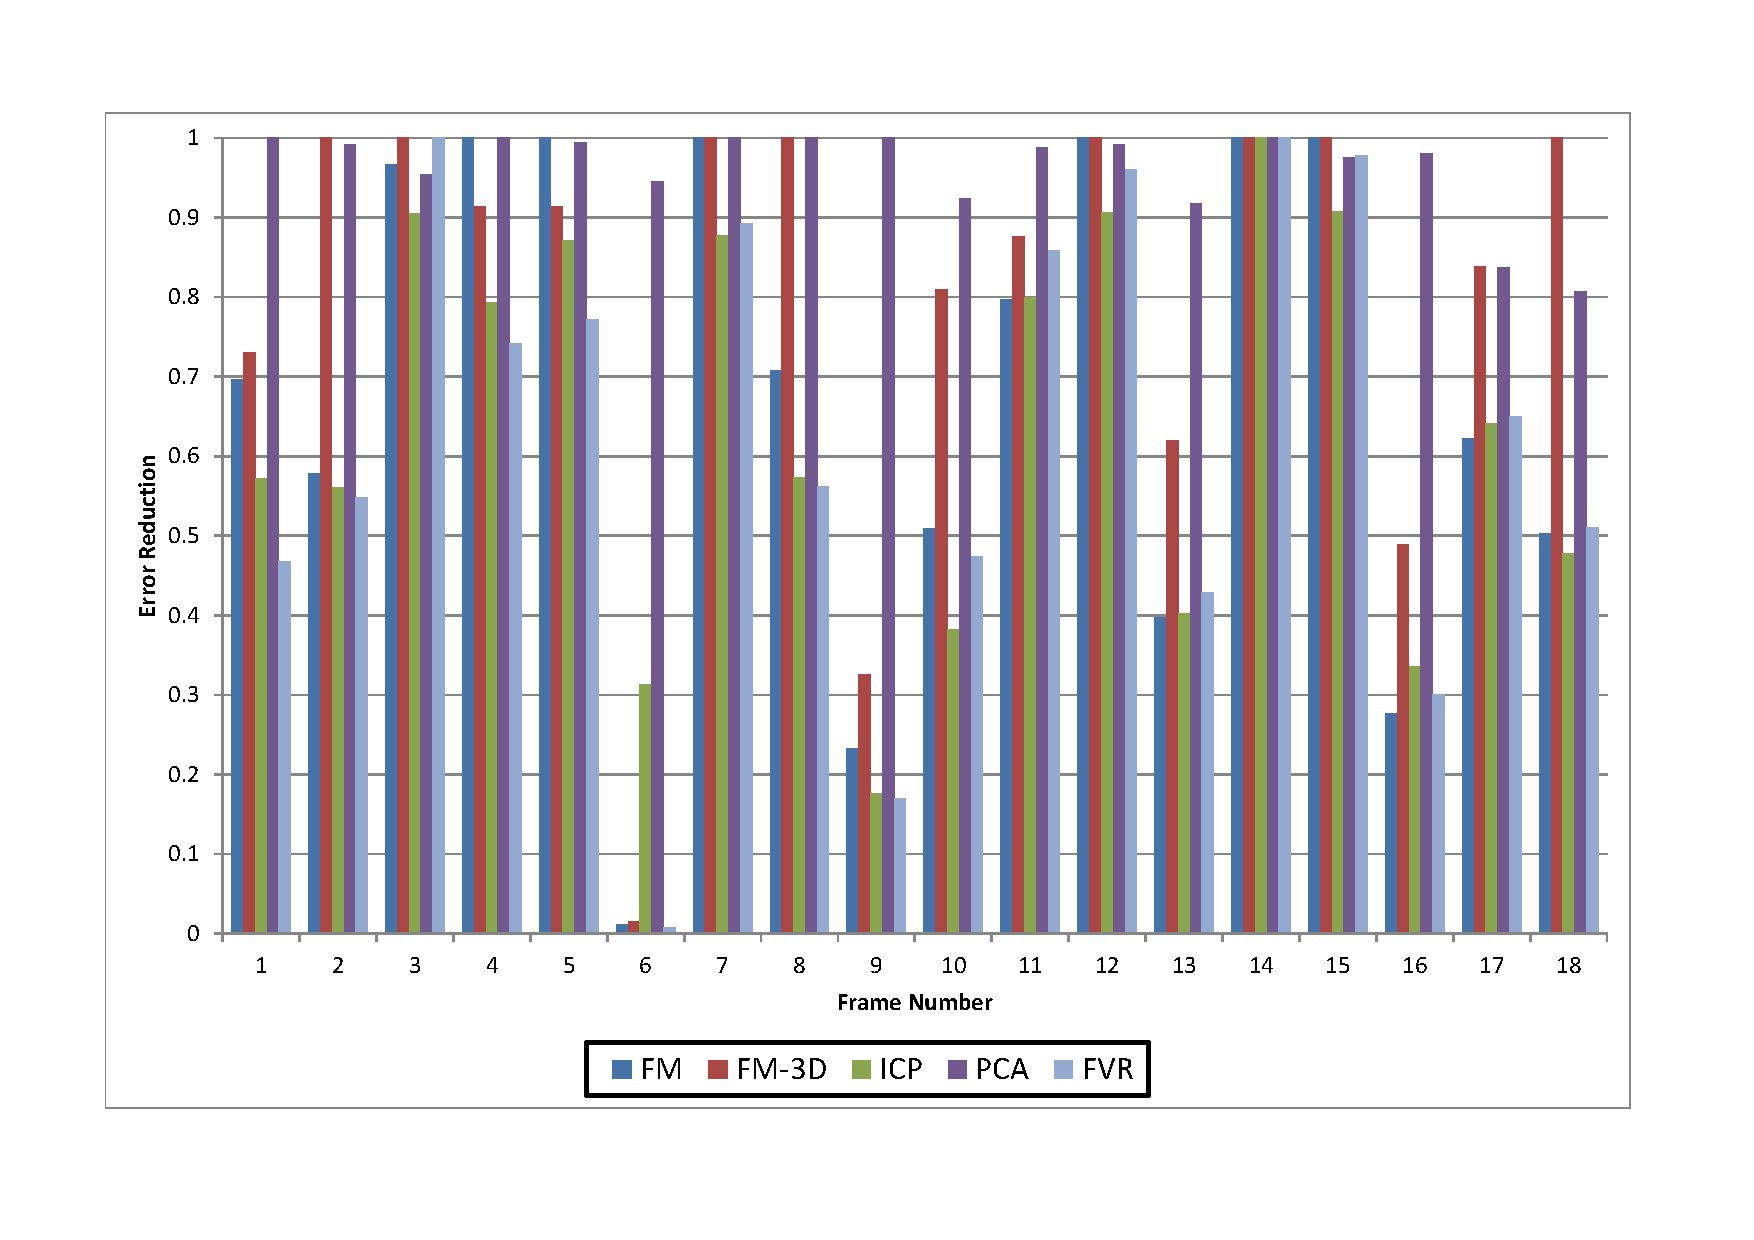
\includegraphics[width=6in]{images/results/IndoorSpace_texture_confusion_translation}
\caption{Registration Error for the Texture Confusion Indoor-Space Translation Data Set}
\label{fig:PET5}

\begin{tabular}{ccc}
\hline
\textbf{Algorithm} & \textbf{Average Error $\times$ 1000} & \textbf{\% best result}\\ \hline
FM-2D	& 715.72 & ~22.22\\
FM-3D	& 992.34 & 0\\
ICP		& 687.31 & ~33.33\\
PCA		& 975.77 & 0\\
FVR		& 630.47 & ~44.44\\
\end{tabular}
\captionof{table}{Statistics for the Texture Confusion Indoor-Space Translation Data Set}
%\label{tab:PET5ST}
\end{figure} 


An important data-set tested is the Indoor-Space with texture confusion (figure \ref{fig:PET5}). Here, a small scene was observed, where texture-confusion was present, this makes registration more difficult for all algorithms most notably the feature matching methods. We suspected that ICP, PCA, and FVR would perform best with this data set. \\

Here, around 44\% of the time, FVR performed best. Additionally it had the lowest average error compared to all the other algorithms. The 2D-FM method achieved the best registration result around 22\% of time, and ICP improved on this at around 33\% of the time. It is clear that 2D-FM and ICP also work quite well but they do not reach the performance of the FVR method. \\ 


%pet 6 Texture Confusion Indoor-Space Translation Data Set
\begin{figure}
\centering
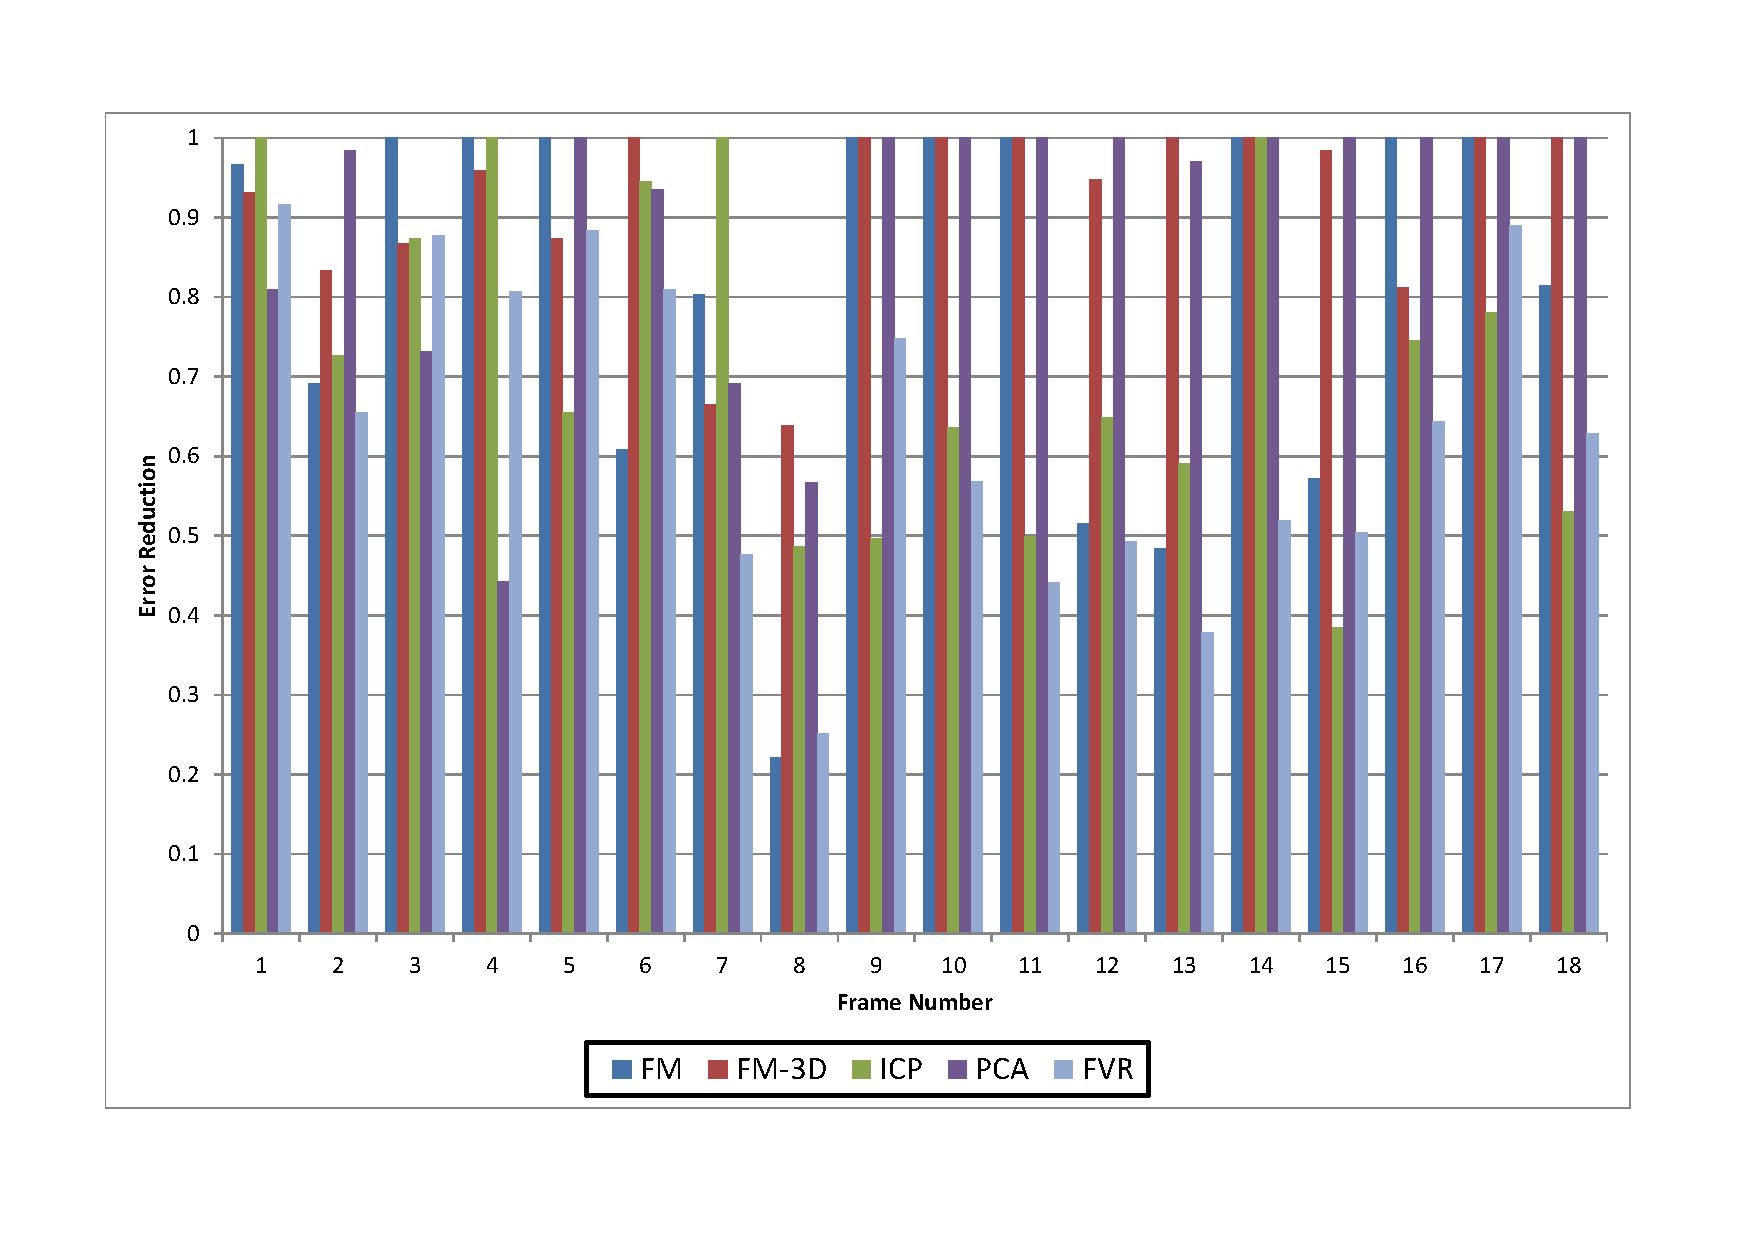
\includegraphics[width=6in]{images/results/Kitchen_LittleTexture_Pan}
\caption{Registration Error for the Low-Texture Kitchen Translation Data Set}
\label{fig:PET6}

\begin{tabular}{ccc}
\hline
\textbf{Algorithm} & \textbf{Average Error $\times$ 1000} & \textbf{\% best result}\\ \hline
FM-2D	& 3450.6 & ~11.11\\
FM-3D	& 973.27 & 0\\
ICP		& 772.9 & ~27.77\\
PCA		& 1029 & ~16.66\\
FVR		& 638.5 & ~44.44\\
\end{tabular}
\captionof{table}{Statistics for the Low-Texture Kitchen Translation Data Set}
%\label{tab:PET6ST}
\end{figure} 


Results for the low-textured Kitchen data-set were collected and shown in figure \ref{fig:PET6}. Again around 44\% of the frames had best results given by FVR. Compared with the next best algorithm ICP at ~27\%. In this case, this is expected as the feature-matching methods should perform worse in a low-textured scene. PCA was next best having the best registration ~22\% of the time. \\


%pet 7 Low-Texture Kitchen Zoom Data Set
\begin{figure}
\centering
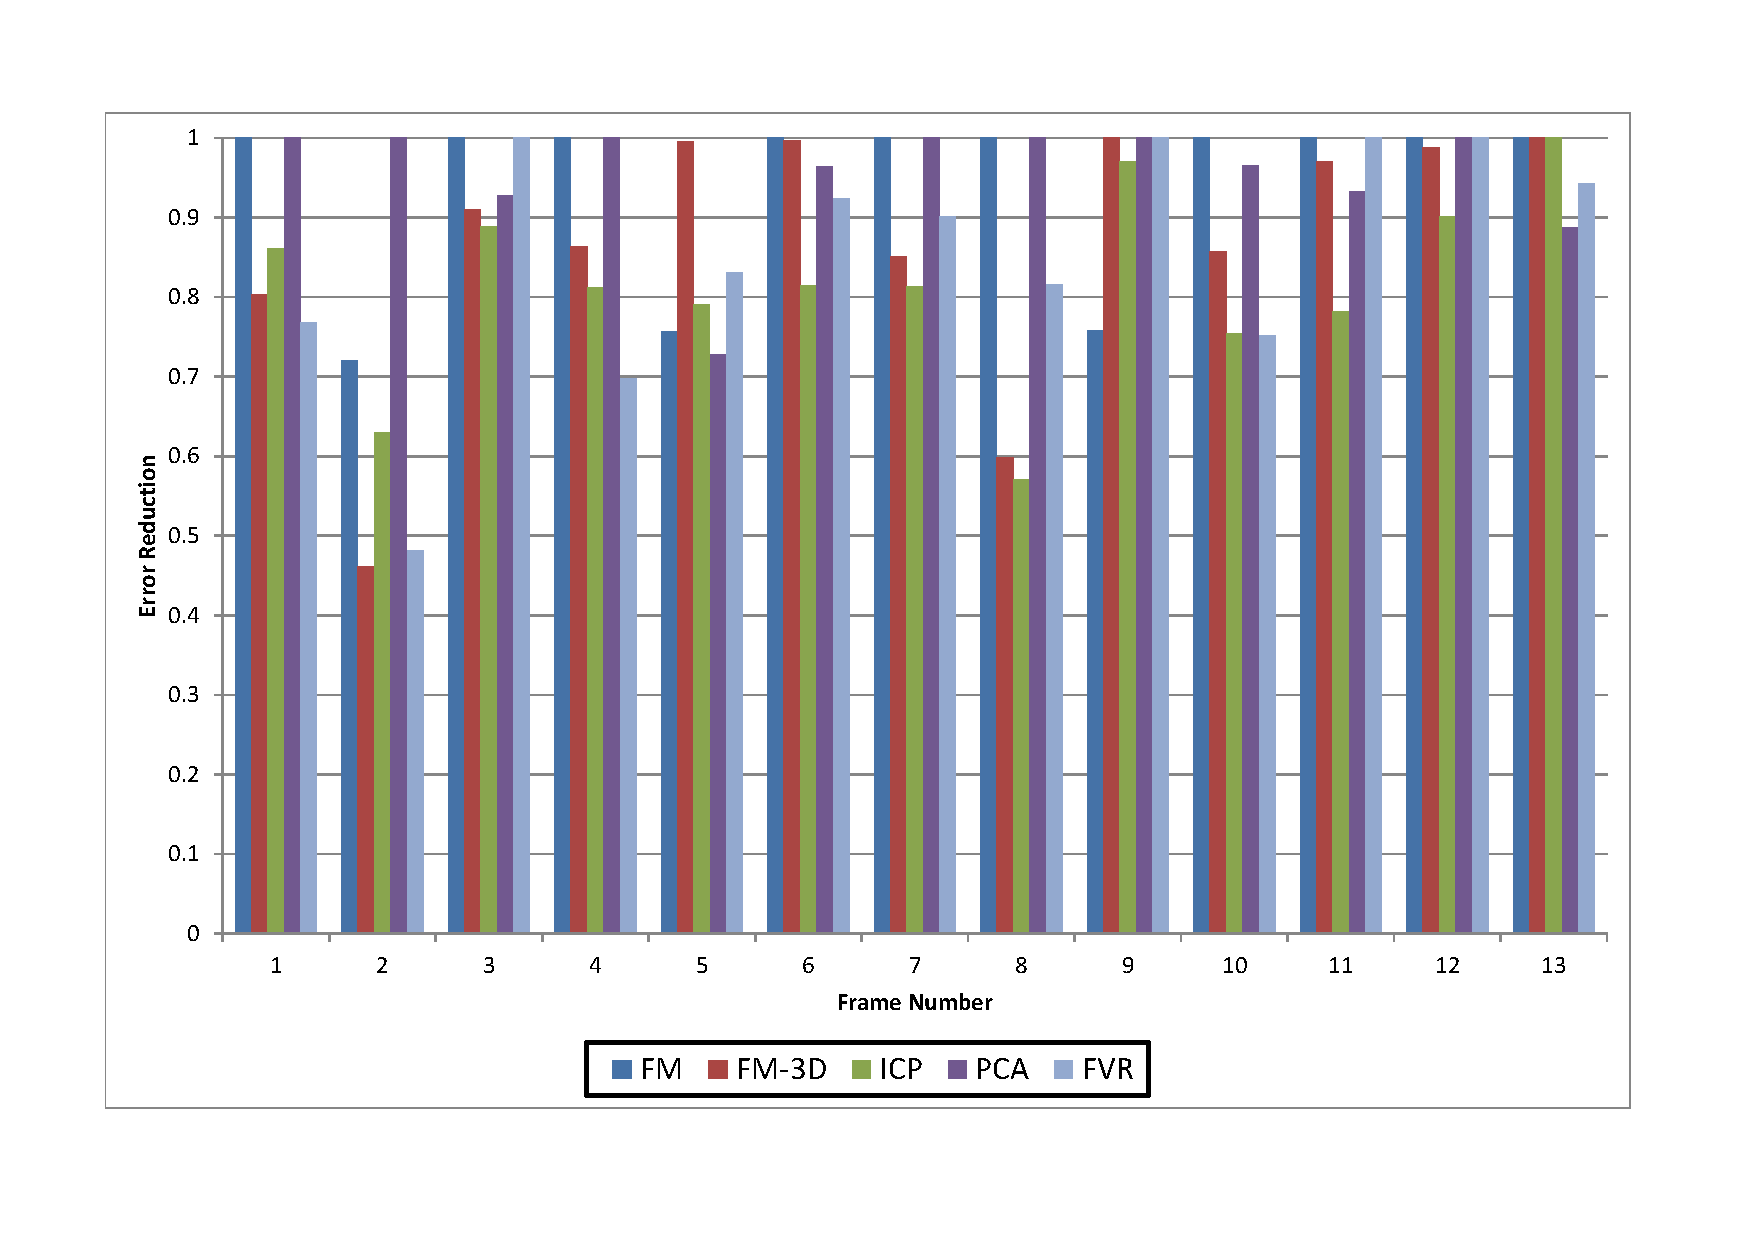
\includegraphics[width=6in]{images/results/Kitchen_Little_Texture_Zoom}
\caption{Registration Error for the Low-Texture Kitchen Zoom Data Set}
\label{fig:PET7}

\begin{tabular}{ccc}
\hline
\textbf{Algorithm} & \textbf{Average Error $\times$ 1000} & \textbf{\% best result}\\ \hline
FM-2D	& 1645.35 & ~7.69\\
FM-3D	& 899.43 & ~7.69\\
ICP		& 833.2 & ~46.15\\
PCA		& 1062.88 & ~15.38\\
FVR		& 875.85 & ~23.08\\
\end{tabular}
\captionof{table}{Statistics for the Low-Texture Kitchen Zoom Data Set}
%\label{tab:PET7ST}
\end{figure} 



Another test for the low-textured Kitchen scene was also performed, this time by moving the camera forward and backwards, zooming in on the scene. In this test, FVR only outperformed the other methods in around 23\% of the frames. ICP outperformed FVR and the other algorithms in around 46\%. Here, FVR performed second best, with an average error performance close to that of ICP. This result is different from the previous result with the low-textured Kitchen scene. There (figure \ref{fig:PET6}), FVR outperformed all of the other methods. This scene is different in that the camera was translated back and forth rather than side to side. Still, the FVR performed competitively compared to the other algorithms.  \\


%pet 8 Office Translation Data Set
\begin{figure}
\centering
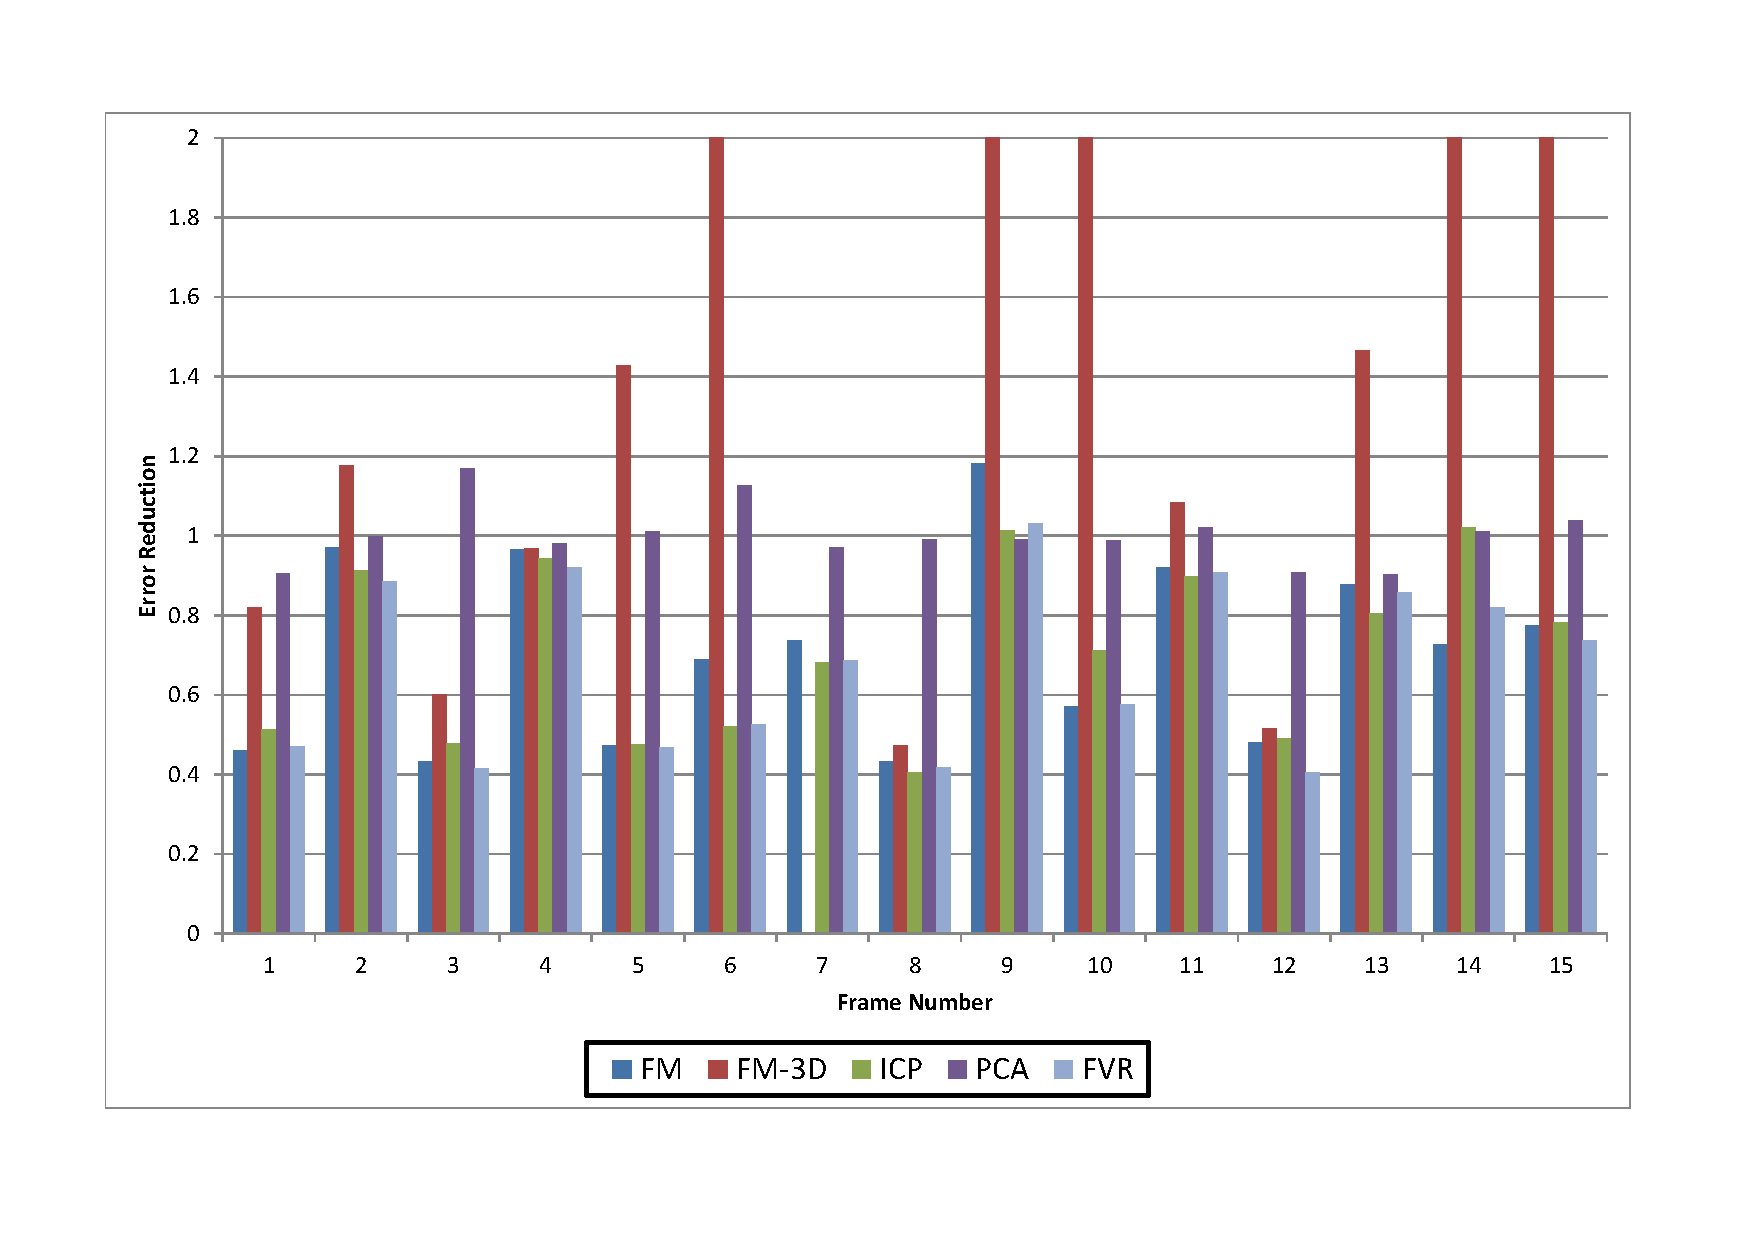
\includegraphics[width=6in]{images/results/Office_TexturedItems_Translation}
\caption{Registration Error for the Office Translation Data Set}
\label{fig:PET8}

\begin{tabular}{ccc}
\hline
\textbf{Algorithm} & \textbf{Average Error $\times$ 1000} & \textbf{\% best result}\\ \hline
FM-2D	& 712.97 & 20\\
FM-3D	& 367040 & 0\\
ICP		& 710.34 & ~33.33\\
PCA		& 1001.43 & ~6.67\\
FVR		& 674.78 & 40\\
\end{tabular}
\captionof{table}{Statistics for the Office Translation Data Set}
%\label{tab:PET8ST}
\end{figure} 


In the results for the Textured Office set (figure \ref{fig:PET8}), FVR matched or beat the other algorithms around 40\% of the time. 2D-feature matching also performed well but did not manage to best FVR most of the time. This result shows that FVR not only works well compared to other algorithms in scenes with little or no texture or in scenes where feature confusion is high, but also in high texture scenes where feature-matching and ICP should have an advantage. The FVR algorithm also had the lowest average registration error compared to these other iterative methods. \\

%pet 9 Office Centered Object Rotation Data Set
\begin{figure}
\centering
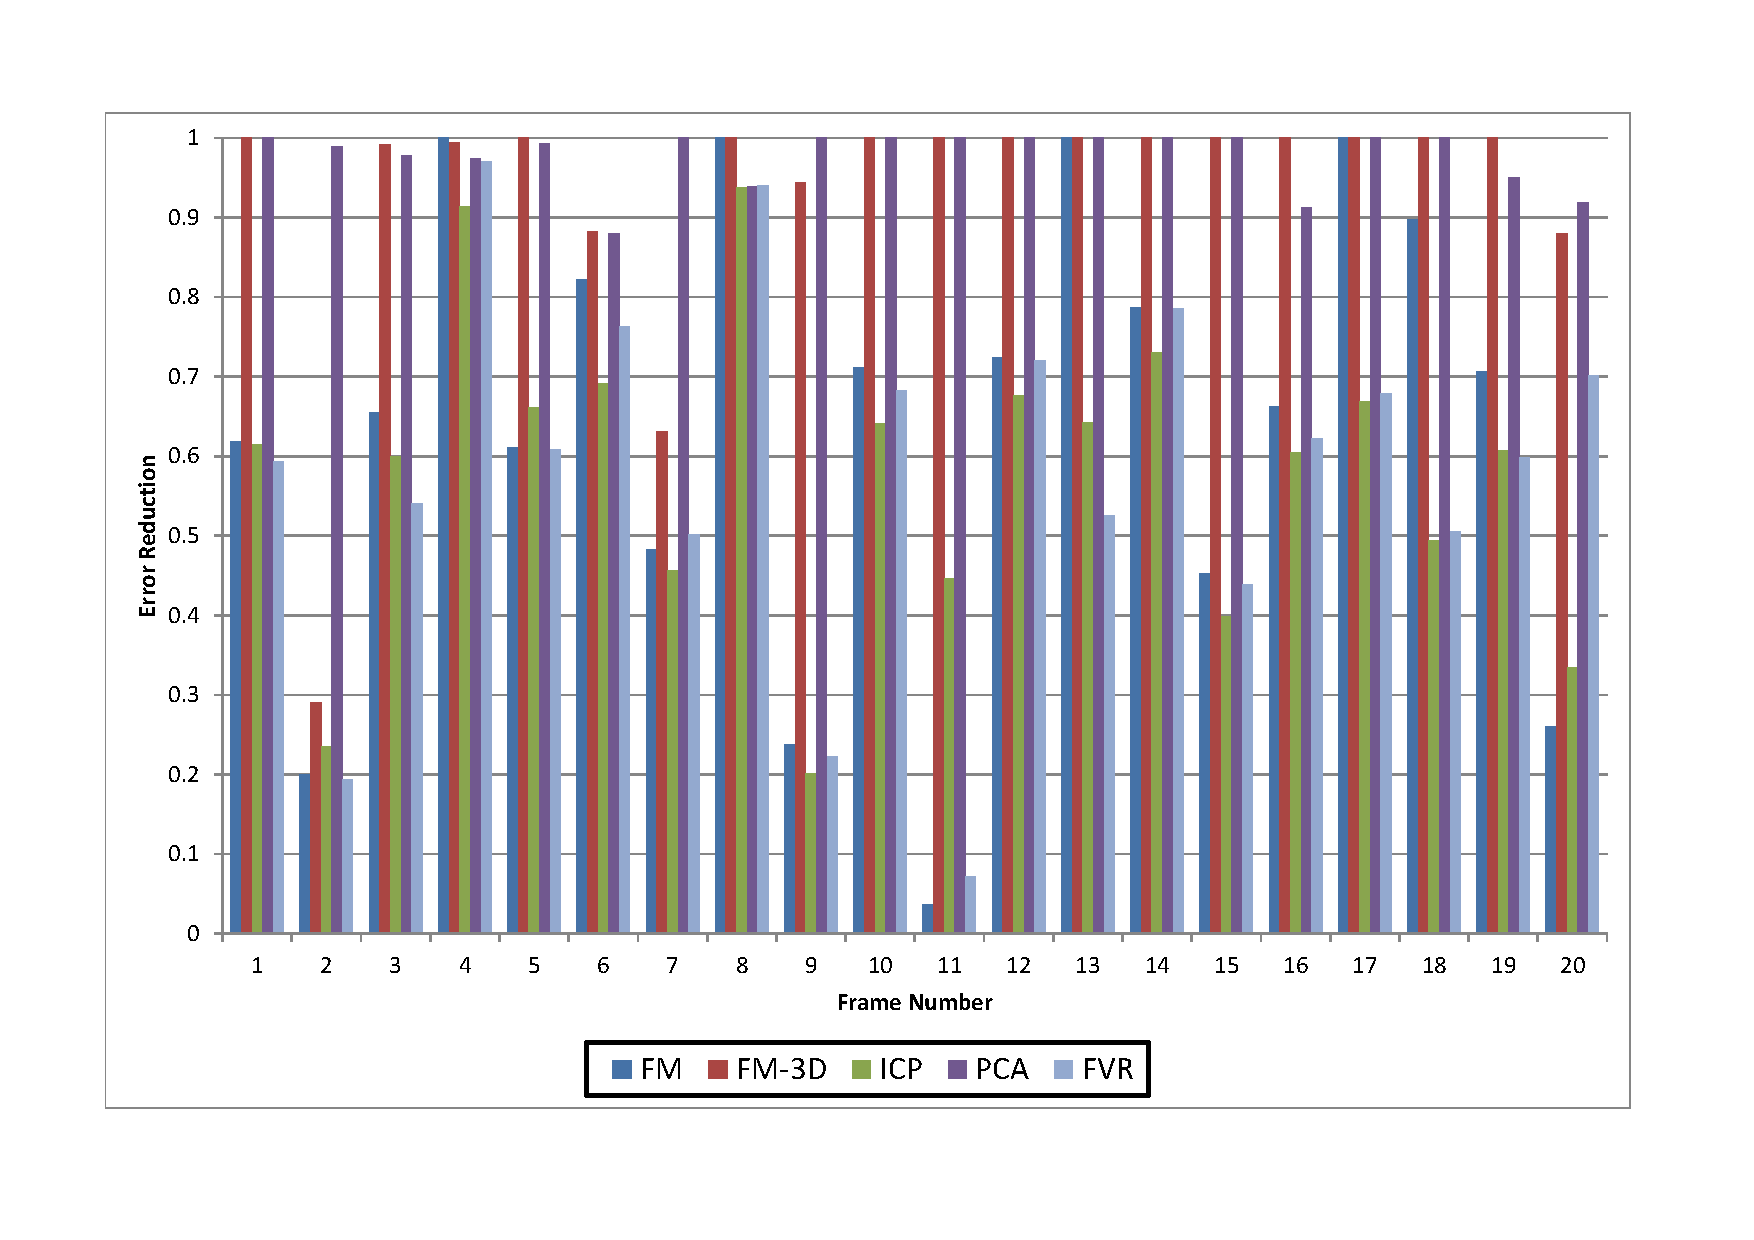
\includegraphics[width=6in]{images/results/Office_Texture_blind_spot_rotation}
\caption{Registration Error for the Office Centered Object Rotation Data Set}
\label{fig:PET9}

\begin{tabular}{ccc}
\hline
\textbf{Algorithm} & \textbf{Average Error $\times$ 1000} & \textbf{\% best result}\\ \hline
FM-2D	& 666.04 & 10\\
FM-3D	& 391310.1 & 0\\
ICP		& 577.93 & 60\\
PCA		& 1026.54 & 0\\
FVR		& 583.42 & 30\\
\end{tabular}
\captionof{table}{Statistics for the Office Centered Object Rotation Data Set}
%\label{tab:PET9ST}
\end{figure} 


Figure \ref{fig:PET9} shows results for the centred object rotation scene. Here, a large divider was placed in the middle of two desks. The idea was to create an environment where the large divider could throw off the effects of PCA and FVR and give an advantage to the feature matching approaches and ICP. Interestingly, around 30\% of the time, FVR had the best result. 2D-feature-matching outperformed the 3D counterpart but only got achieved the best registration performance around 10\% of the time. ICP on the other hand got the best result for around 60\% of the frames. In this scene ICP is able to use the large divider as an anchor which would make it more robust to non-overlapped data.

%pet 10 Office X/Y-Axis Rotation Data Set
\begin{figure}
\centering
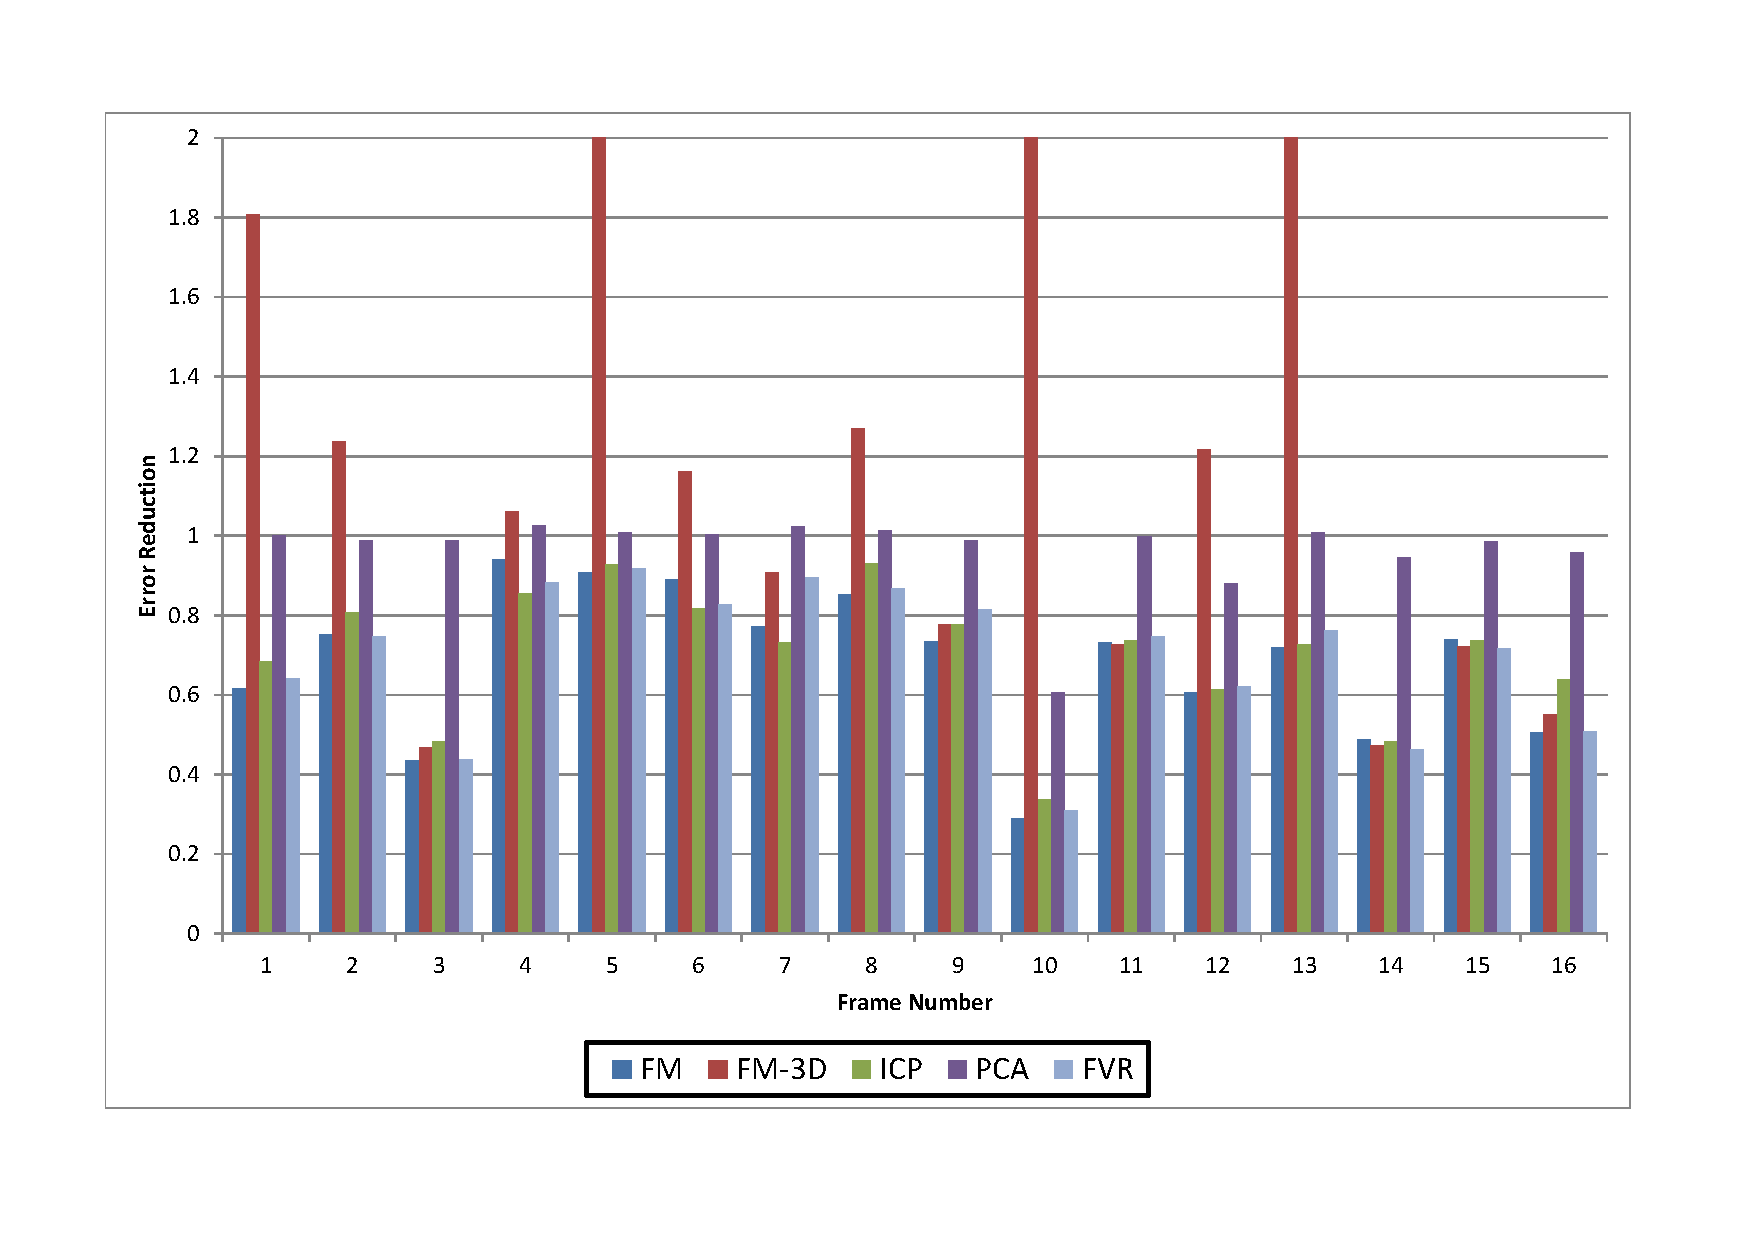
\includegraphics[width=6in]{images/results/Office_Texture_Rotate_XAxis}
\caption{Registration Error for the Office X/Y-Axis Rotation Data Set}
\label{fig:PET10}

\begin{tabular}{ccc}
\hline
\textbf{Algorithm} & \textbf{Average Error $\times$ 1000} & \textbf{\% best result}\\ \hline
FM-2D	& 686.48 & ~56.25\\
FM-3D	& 2080.65 & ~6.25\\
ICP		& 705.76 & ~18.75\\
PCA		& 964.13 & 0\\
FVR		& 697.27 & ~18.75\\
\end{tabular}
\captionof{table}{Statistics for the Office X/Y-Axis Rotation Data Set}
%\label{tab:PET10ST}
\end{figure} 


Another experiment where the scene was filmed with the camera rotated predominantly about the x-axis is shown in figure \ref{fig:PET10}, this time 2D-feature-matching outperformed the others. FVR and ICP performed second best in terms of the percent of best results achieved but FVR had a lower average registration error which came close to beating FM-2D.  

%pet 11 Office Y-Axis Rotation Data Set
\begin{figure}
\centering
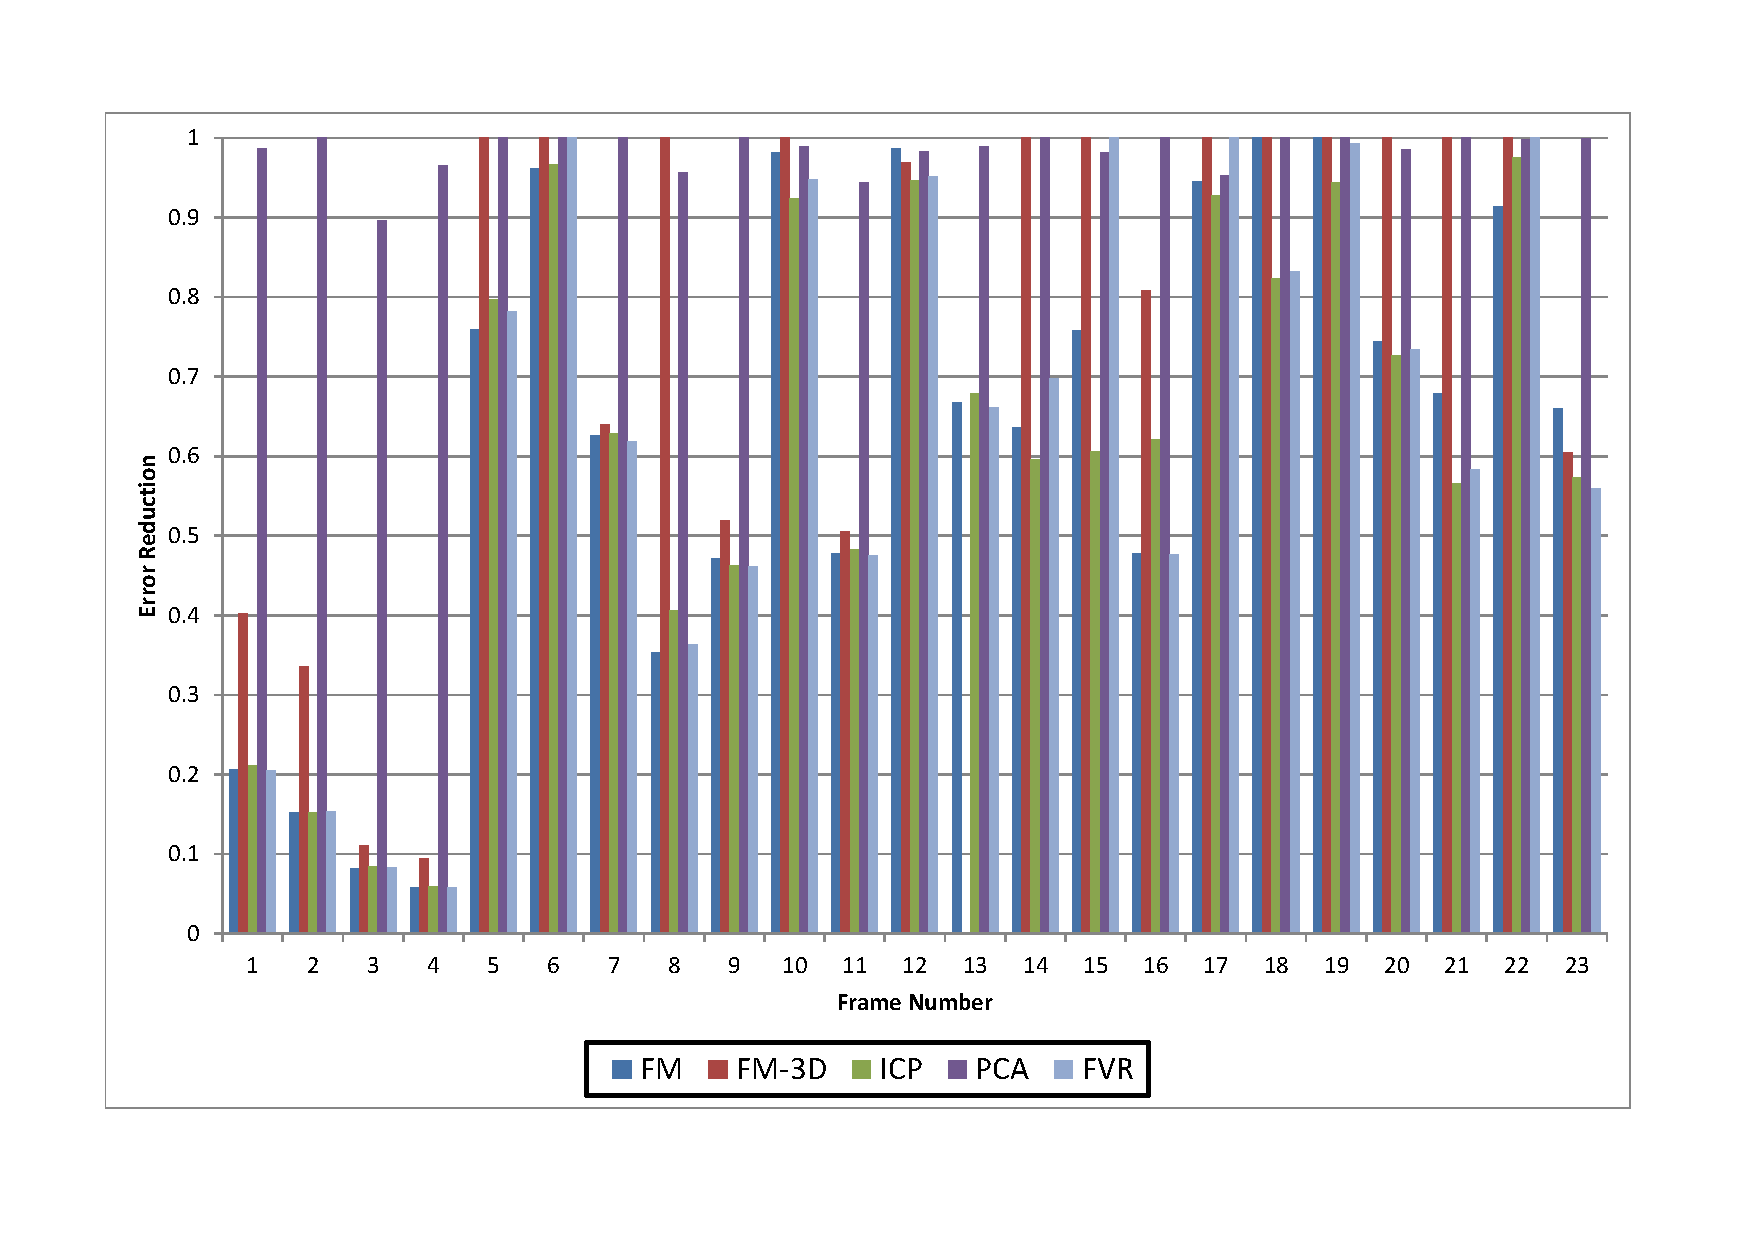
\includegraphics[width=6in]{images/results/Office_Texture_Rotation}
\caption{Registration Error for the Office Y-Axis Rotation Data Set}
\label{fig:PET11}

\begin{tabular}{ccc}
\hline
\textbf{Algorithm} & \textbf{Average Error $\times$ 1000} & \textbf{\% best result}\\ \hline
FM-2D	& 530 & ~35.71\\
FM-3D	& 934.53 & 0\\
ICP		& 528.47 & ~28.57\\
PCA		& 1000.78 & 0\\
FVR		& 533.23 & ~35.71\\
\end{tabular}
\captionof{table}{Statistics for the Office Y-Axis Rotation Data Set}
%\label{tab:PET11ST}
\end{figure} 


Figure \ref{fig:PET11} shows the registration errors for the Office data-set with camera rotation about the Y-axis. Here, in around 35\% of the cases, FVR outperformed the other algorithms. This result matched the 2D feature matching method. Both the FVR and 2D-FM method achieved a very similar average registration error. ICP actually achieved the lowest average error but did not achieve as high a percentage of optimal results as compared to FVR and FM-2D. \\

%pet 12 Office Translation Data Set
\begin{figure}
\centering
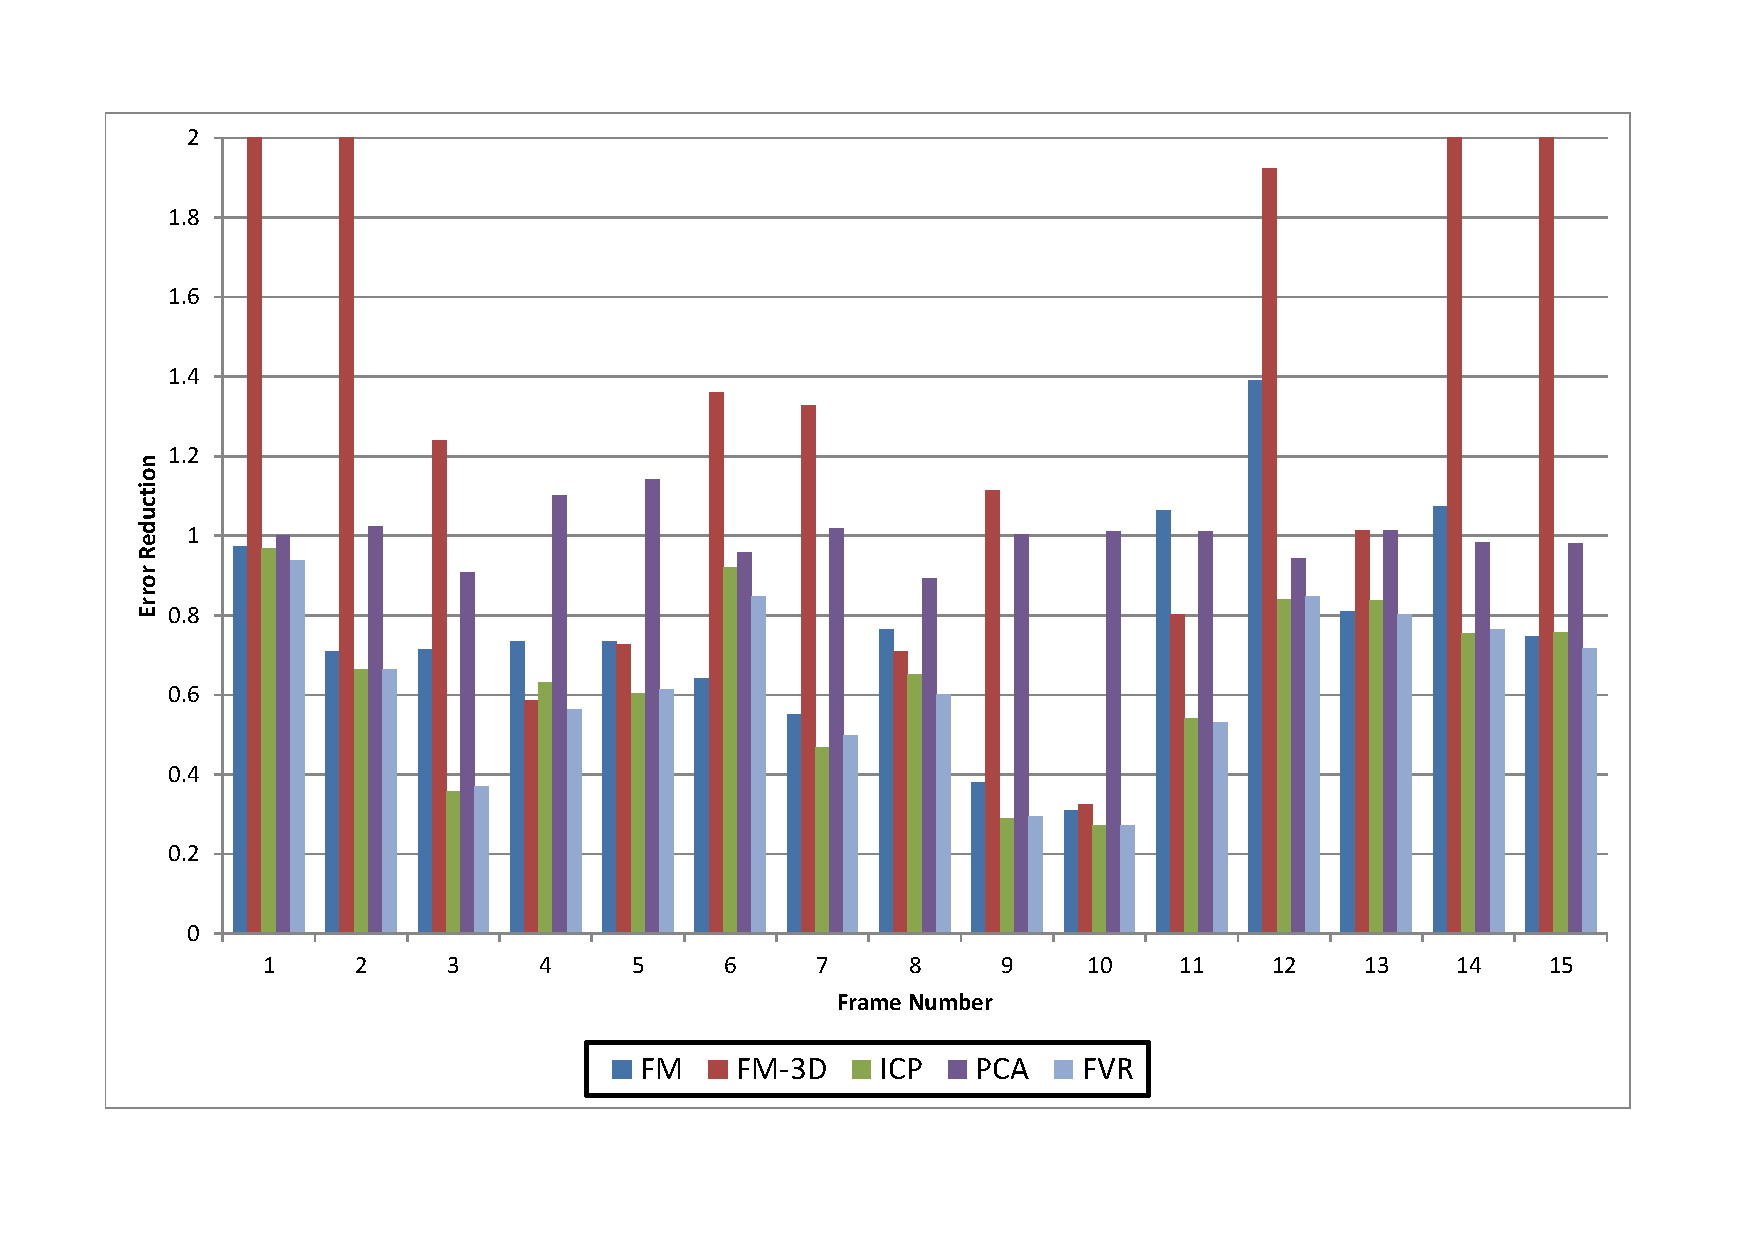
\includegraphics[width=6in]{images/results/Office_Texture_Translation}
\caption{Registration Error for the Office Translation Data Set}
\label{fig:PET12}

\begin{tabular}{ccc}
\hline
\textbf{Algorithm} & \textbf{Average Error $\times$ 1000} & \textbf{\% best result}\\ \hline
FM-2D	& 773.23 & ~6.67\\
FM-3D	& 2696.51 & 0\\
ICP		& 636.84 & 40\\
PCA		& 999.57 & 0\\
FVR		& 621.72 & ~53.33\\
\end{tabular}
\captionof{table}{Statistics for the Office Translation Data Set}
%\label{tab:PET12ST}
\end{figure} 


In the Office translation scene (figure \ref{fig:PET12}), FVR outperformed or matched the other algorithms around 53\% of the time. It also had the lowest average registration error. This shows that the FVR has high accuracy when dealing with translation detection and the registration of 3D data with only translational changes. Here, PCA and 2D and 3D feature matching performed the worst with ICP performing second best. \\

%pet 13 Little Texture Outdoors Rotation Data Set
\begin{figure}
\centering
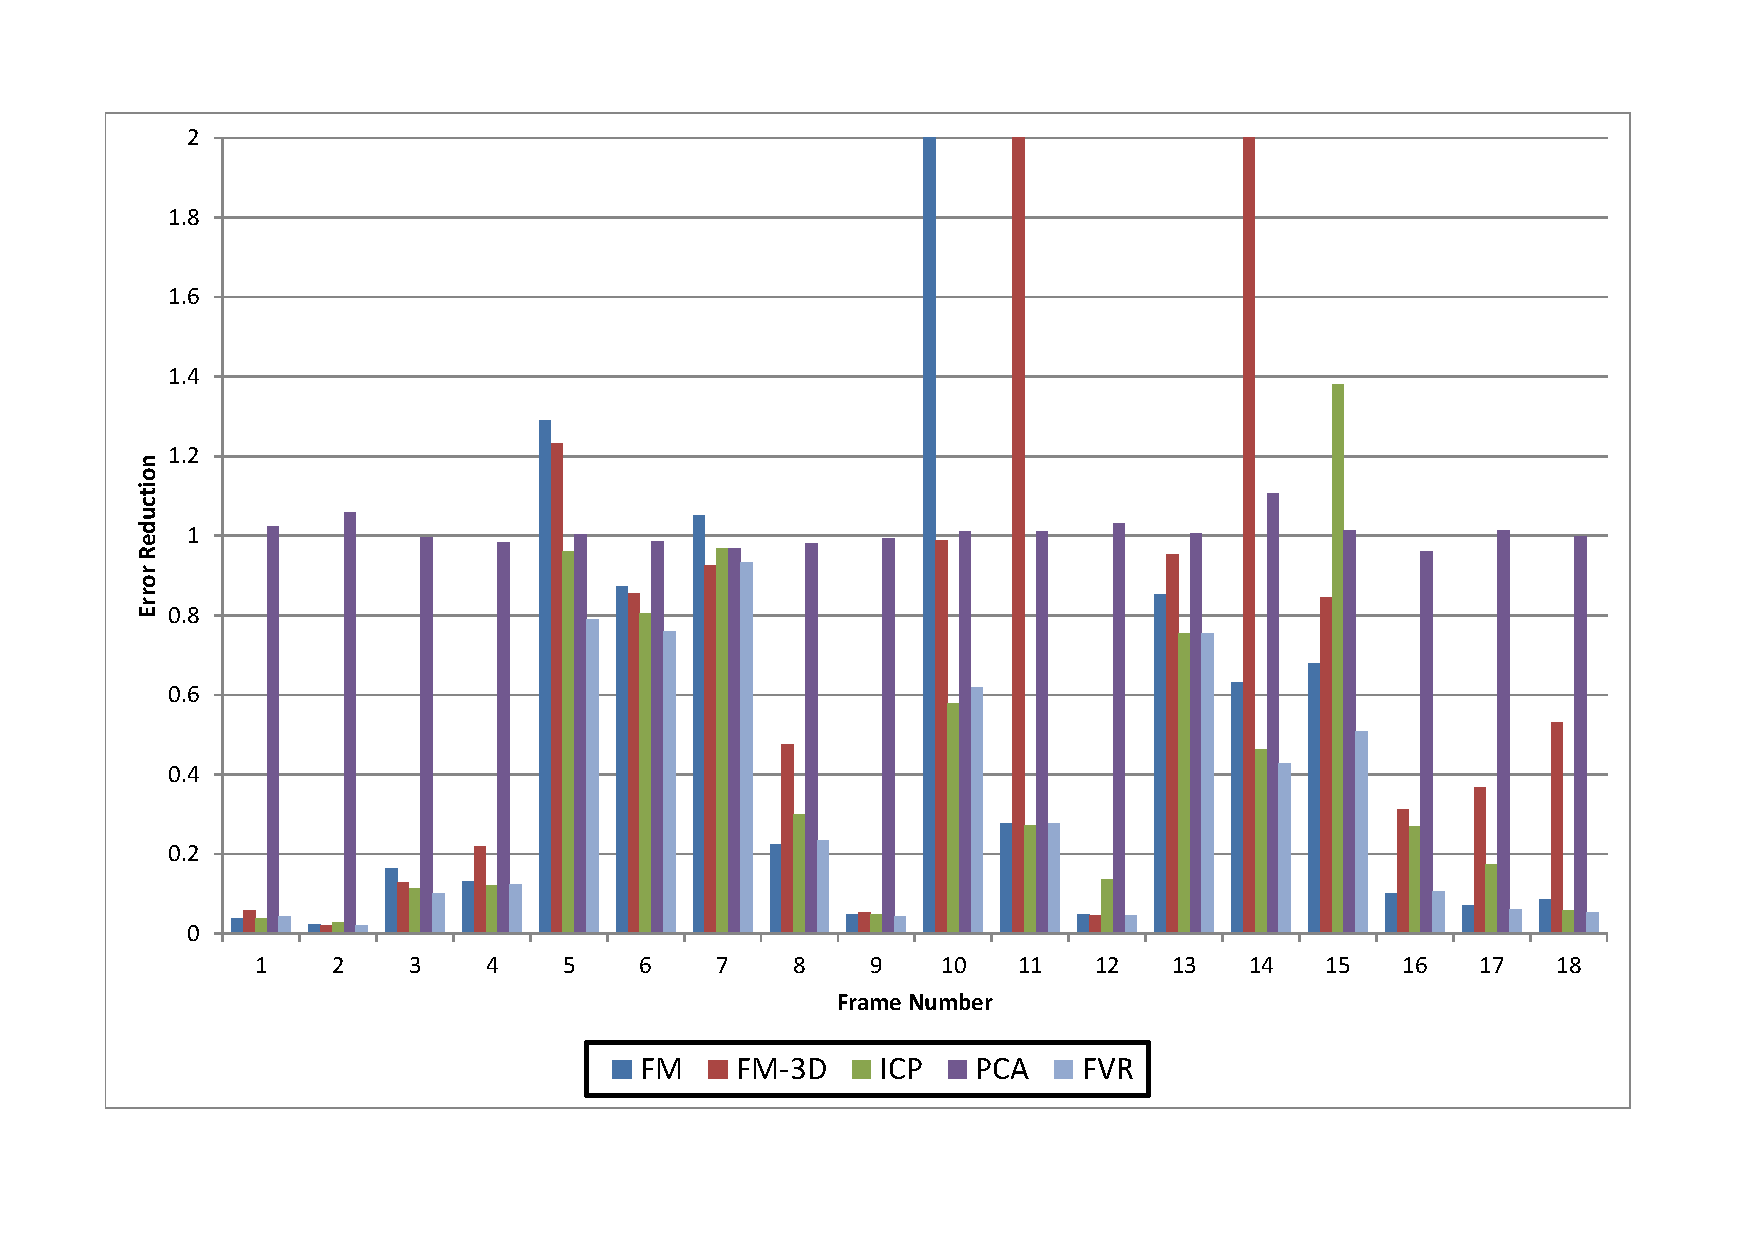
\includegraphics[width=6in]{images/results/Outside_No_Texture_Rotation}
\caption{Registration Error for the Little Texture Outdoors Rotation Data Set}
\label{fig:PET13}

\begin{tabular}{ccc}
\hline
\textbf{Algorithm} & \textbf{Average Error $\times$ 1000} & \textbf{\% best result}\\ \hline
FM-2D	& 497.83 & ~11.11\\
FM-3D	& 12411.23 & ~5.56\\
ICP		& 414.87 & ~27.78\\
PCA		& 1008.22 & 0\\
FVR		& 327.95 & ~55.56\\
\end{tabular}
\captionof{table}{Statistics for the Little Texture Outdoors Rotation Data Set}
%\label{tab:PET13ST}
\end{figure} 


Figure \ref{fig:PET13} shows results for an outdoors scene with little texture, here the camera was rotated about an origin. In this case, PCA performed the worst, and 3D-feature-matching also failed several times. FVR again had the largest percent of optimal results, and achieved the lowest average registration error by a considerable margin. This results can be explained by FVR's robustness to out-door scenes and scenes with little to no texture information.  \\

%pet 14 Little Texture Outdoors Rotation Data Set
\begin{figure}
\centering
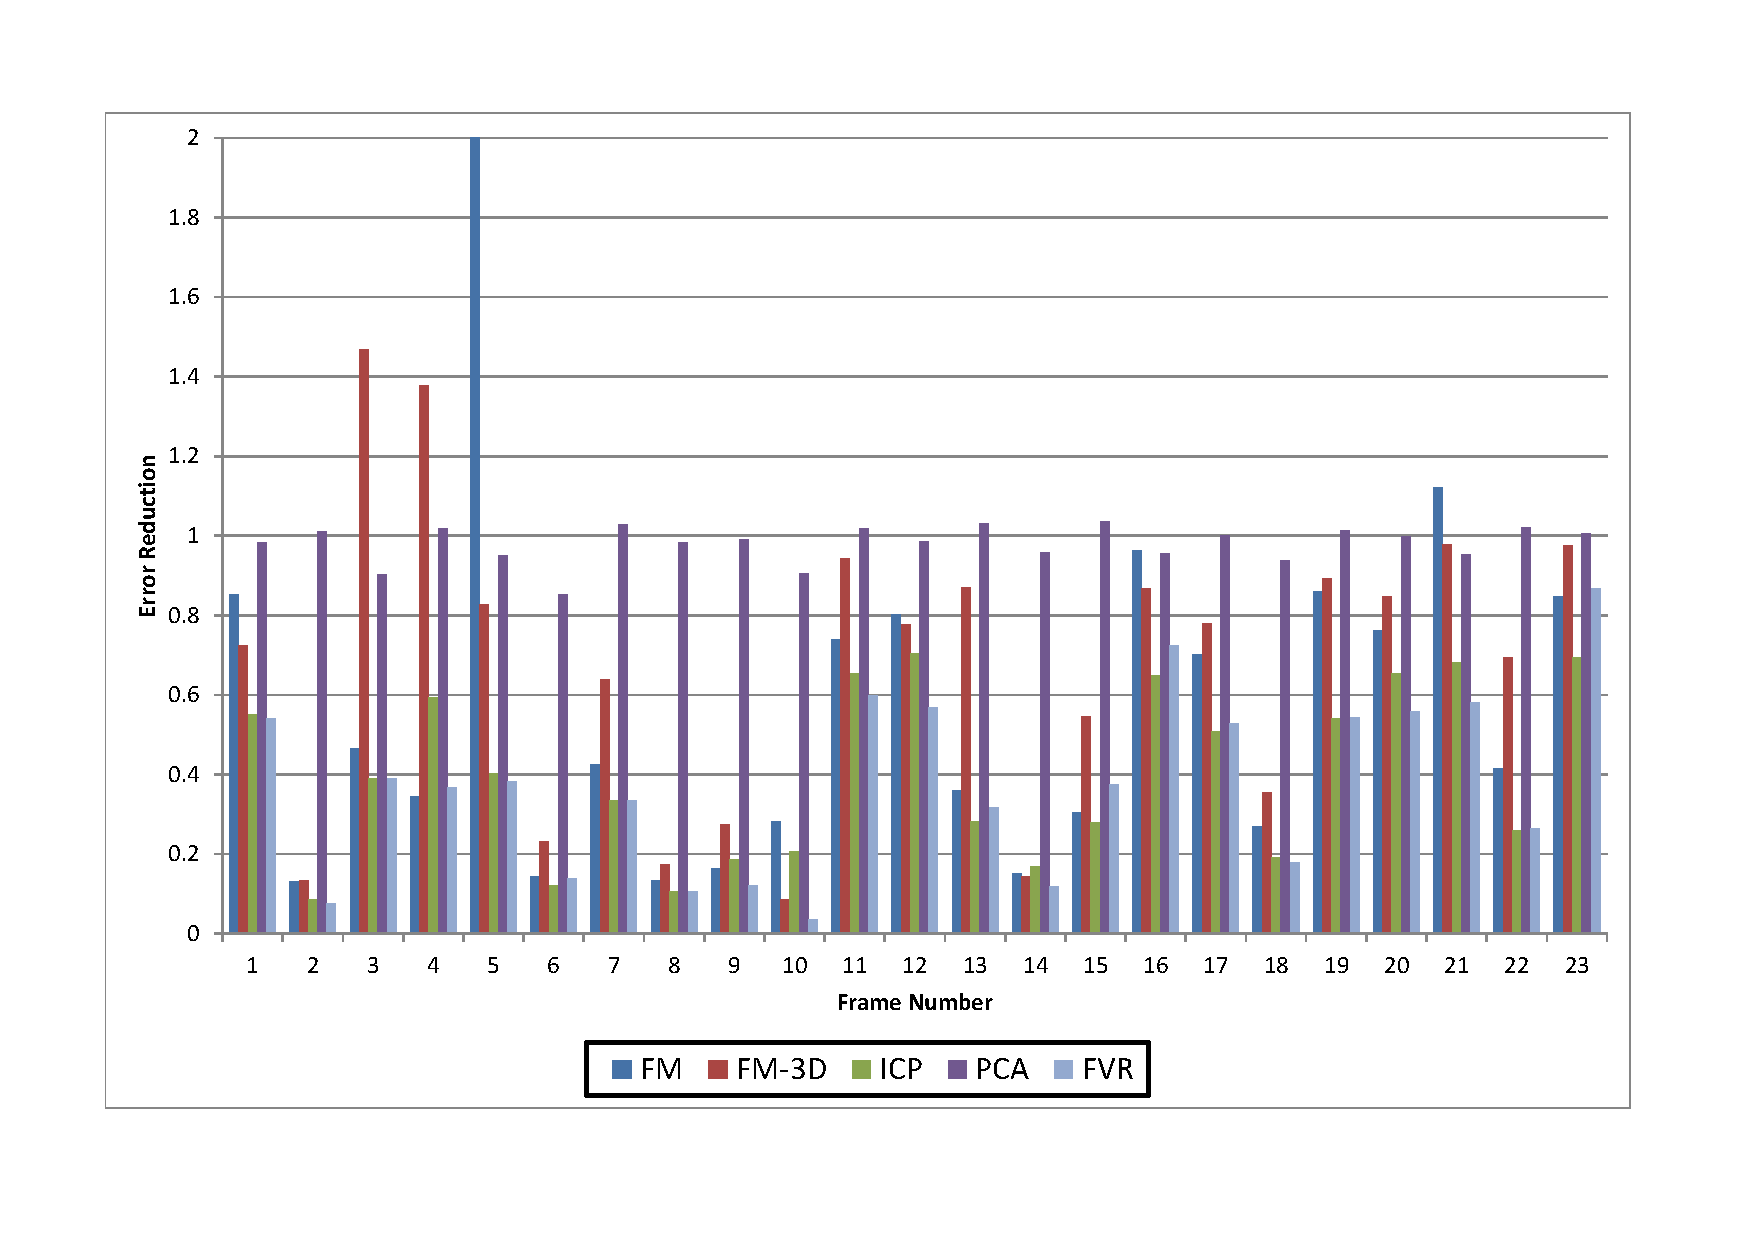
\includegraphics[width=6in]{images/results/Outside_No_Texture_Translation}
\caption{Registration Error for the Little Texture Outdoors Translation Data Set}
\label{fig:PET14}

\begin{tabular}{ccc}
\hline
\textbf{Algorithm} & \textbf{Average Error $\times$ 1000} & \textbf{\% best result}\\ \hline
FM-2D	& 716.1 & ~4.35\\
FM-3D	& 678.65 & 0\\
ICP		& 402.16 & ~39.13\\
PCA		& 980.15 & 0\\
FVR		& 379.06 & ~56.52\\
\end{tabular}
\captionof{table}{Statistics for the Little Texture Outdoors Translation Data Set}
\label{tab:PET14ST}
\end{figure} 

Another test using a low-textured out-doors scene was tested where the camera was translated along a path. Results are shown in figure \ref{fig:PET14}. Here again the FVR method dominated recording the best result for around 57\% of the frames. Notably, PCA performed poorly despite being a part of the FVR method. This scene was also a rare case where FM-3D outperformed the 2D feature matching version. ICP was more consistent, recoding the best result around 40\% of the time. Again, this shows the strength of the FVR method in out-door and low-texture environments. 


%pet 15 Little Texture Outdoors Rotation Data Set
\begin{figure}
\centering
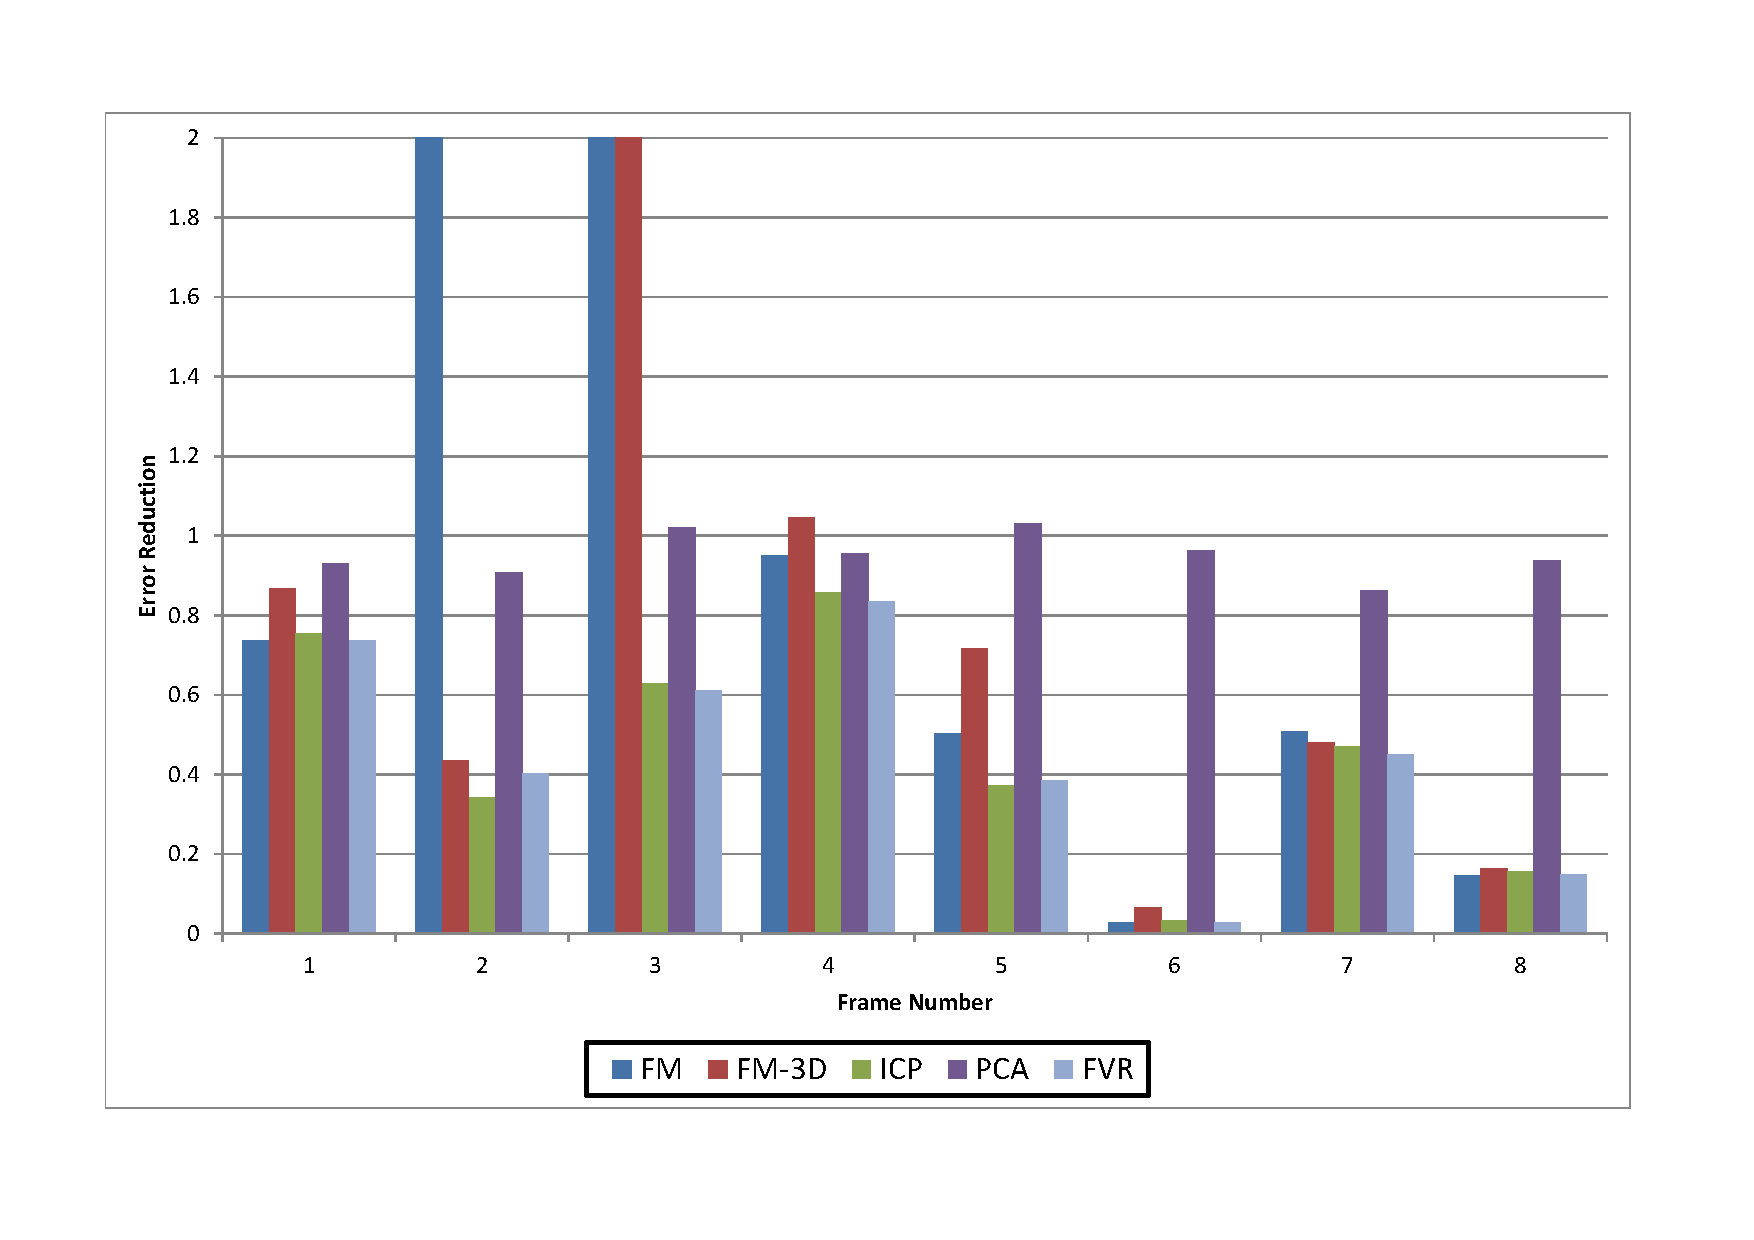
\includegraphics[width=6in]{images/results/Outside_TextureConfusion_Rotation}
\caption{Registration Error for the Outdoors Texture Confusion Rotation Data Set}
\label{fig:PET15}

\begin{tabular}{ccc}
\hline
\textbf{Algorithm} & \textbf{Average Error $\times$ 1000} & \textbf{\% best result}\\ \hline
FM-2D	& 1274.19 & 12.5\\
FM-3D	& 2336.98 & 0\\
ICP		& 452.08 & 25\\
PCA		& 951.42 & 0\\
FVR		& 450.07 & 62.5\\
\end{tabular}
\captionof{table}{Statistics for the Outdoors Texture Confusion Rotation Data Set}
%\label{tab:PET15ST}
\end{figure}


Another test was performed with an outdoors scene. Here only 8 of the frames had any good results for all algorithms as the scene was very difficult to register due to the amount of noise and texture confusion in the captured frames. Results are shown in figure \ref{fig:PET15}. In them the FVR achieved the best result in around 63\% of the frames. 2D-feature-matching and 3D-feature-matching both failed to register a few of these frames, and PCA was inconsistent. ICP had a competitive result but the FVR algorithm still had a lower average registration error. \\ 


%pet 16 Outdoors Texture Confusion Translation Data Set
\begin{figure}
\centering
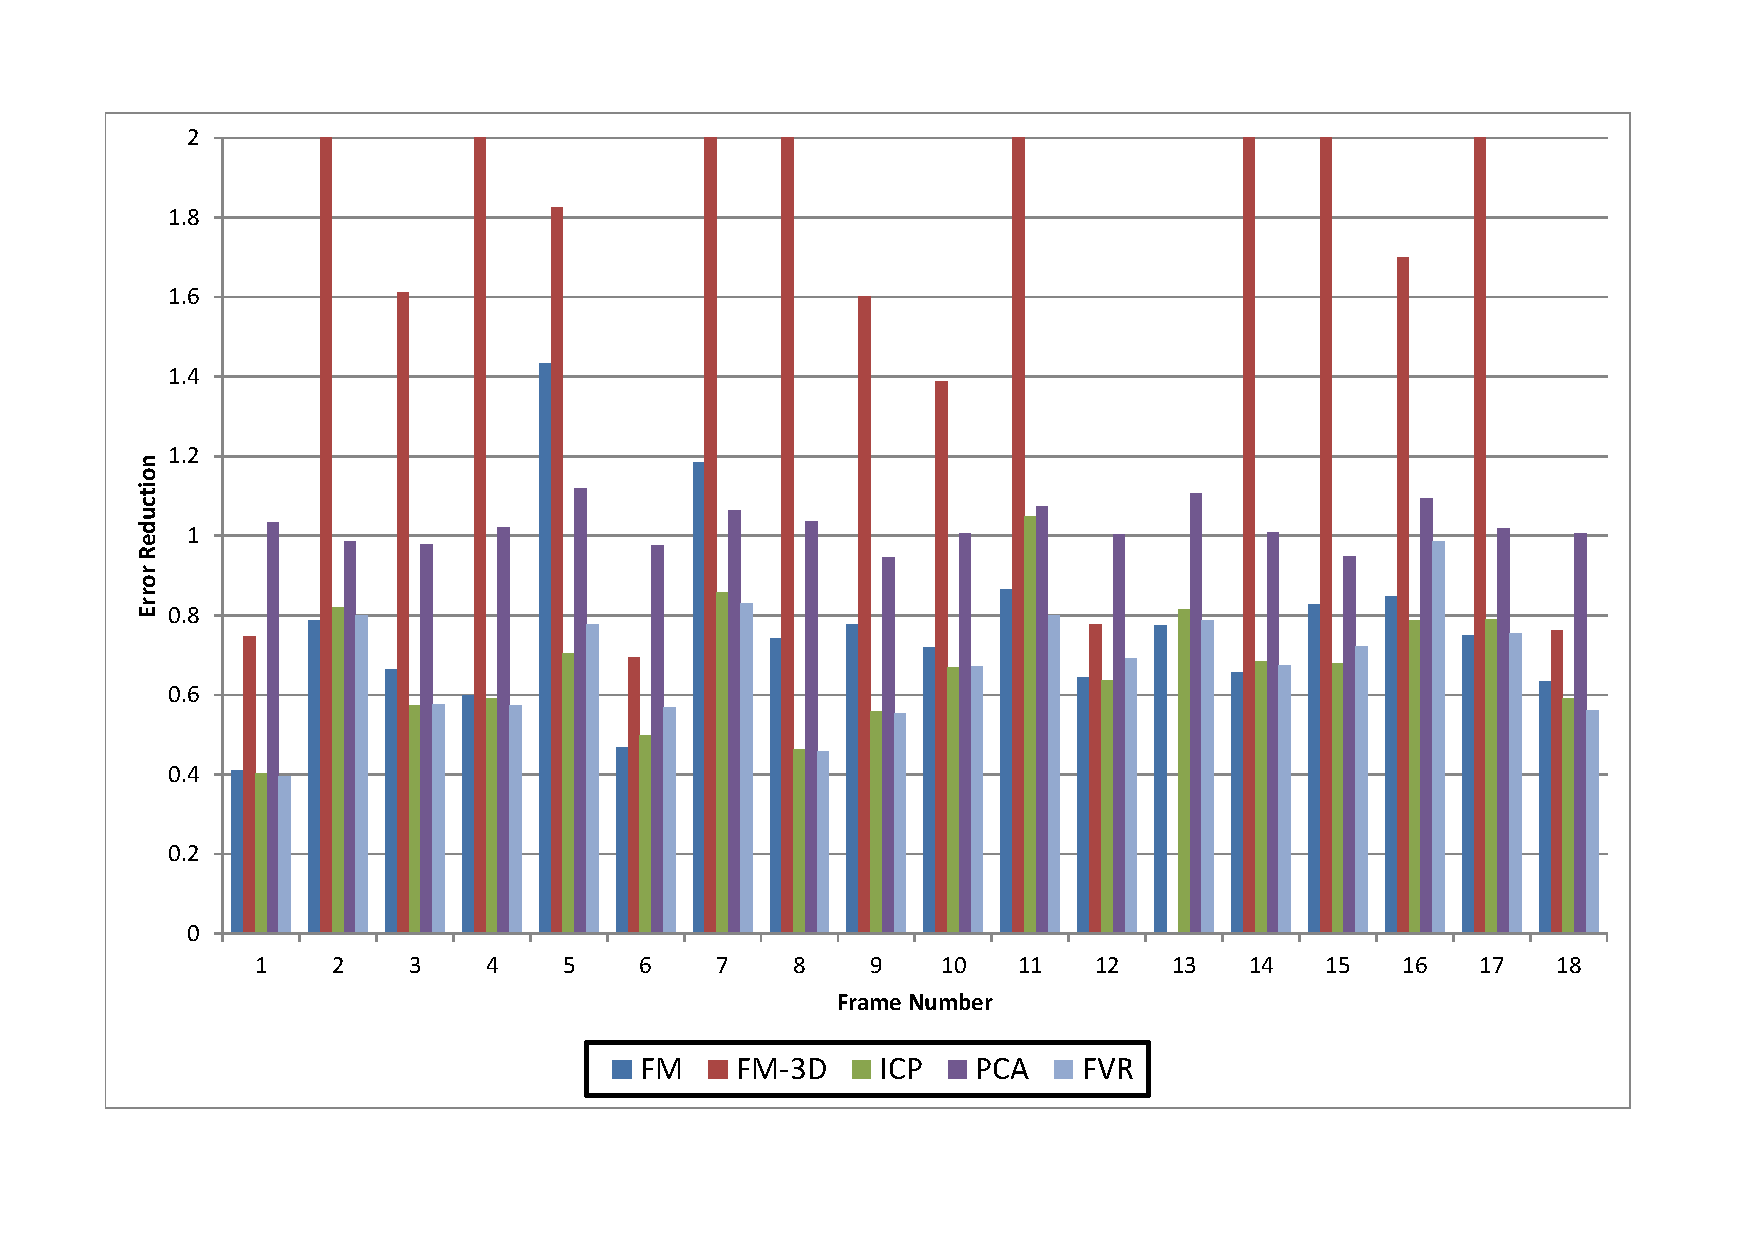
\includegraphics[width=6in]{images/results/Outside_TextureConfusion_Translation}
\caption{Registration Error for the Outdoors Texture Confusion Translation Data Set}
\label{fig:PET16}

\begin{tabular}{ccc}
\hline
\textbf{Algorithm} & \textbf{Average Error $\times$ 1000} & \textbf{\% best result}\\ \hline
FM-2D	& 765.94 & ~27.78\\
FM-3D	& 375694.14 & 0\\
ICP		& 676.02 & ~33.33\\
PCA		& 1023.48 & 0\\
FVR		& 676.51 & ~38.89\\
\end{tabular}
\captionof{table}{Statistics for the Outdoors Texture Confusion Translation Data Set}
%\label{tab:PET16ST}
\end{figure}

Another scene with texture-confusion was taken out-doors. The accompanying results are shown in figure \ref{fig:PET16}. Here, 3D-feature matching failed a majority of the time and thus had a large average registration error. PCA performed poorly due of the amount of noise in this out-doors scene. This noise can give inconsistencies in the principal axes and mean computation. Despite this the FVR again outperformed the other algorithms in terms of the percentage of optimal registrations. Despite this, both ICP's and FVR's average error was a close tie. But because of the percentage of best results achieved by FVR, it is considered to have performed best. \\

%pet 17 Outdoor Plants Texture Confusion Rotation Data Set
\begin{figure}
\centering
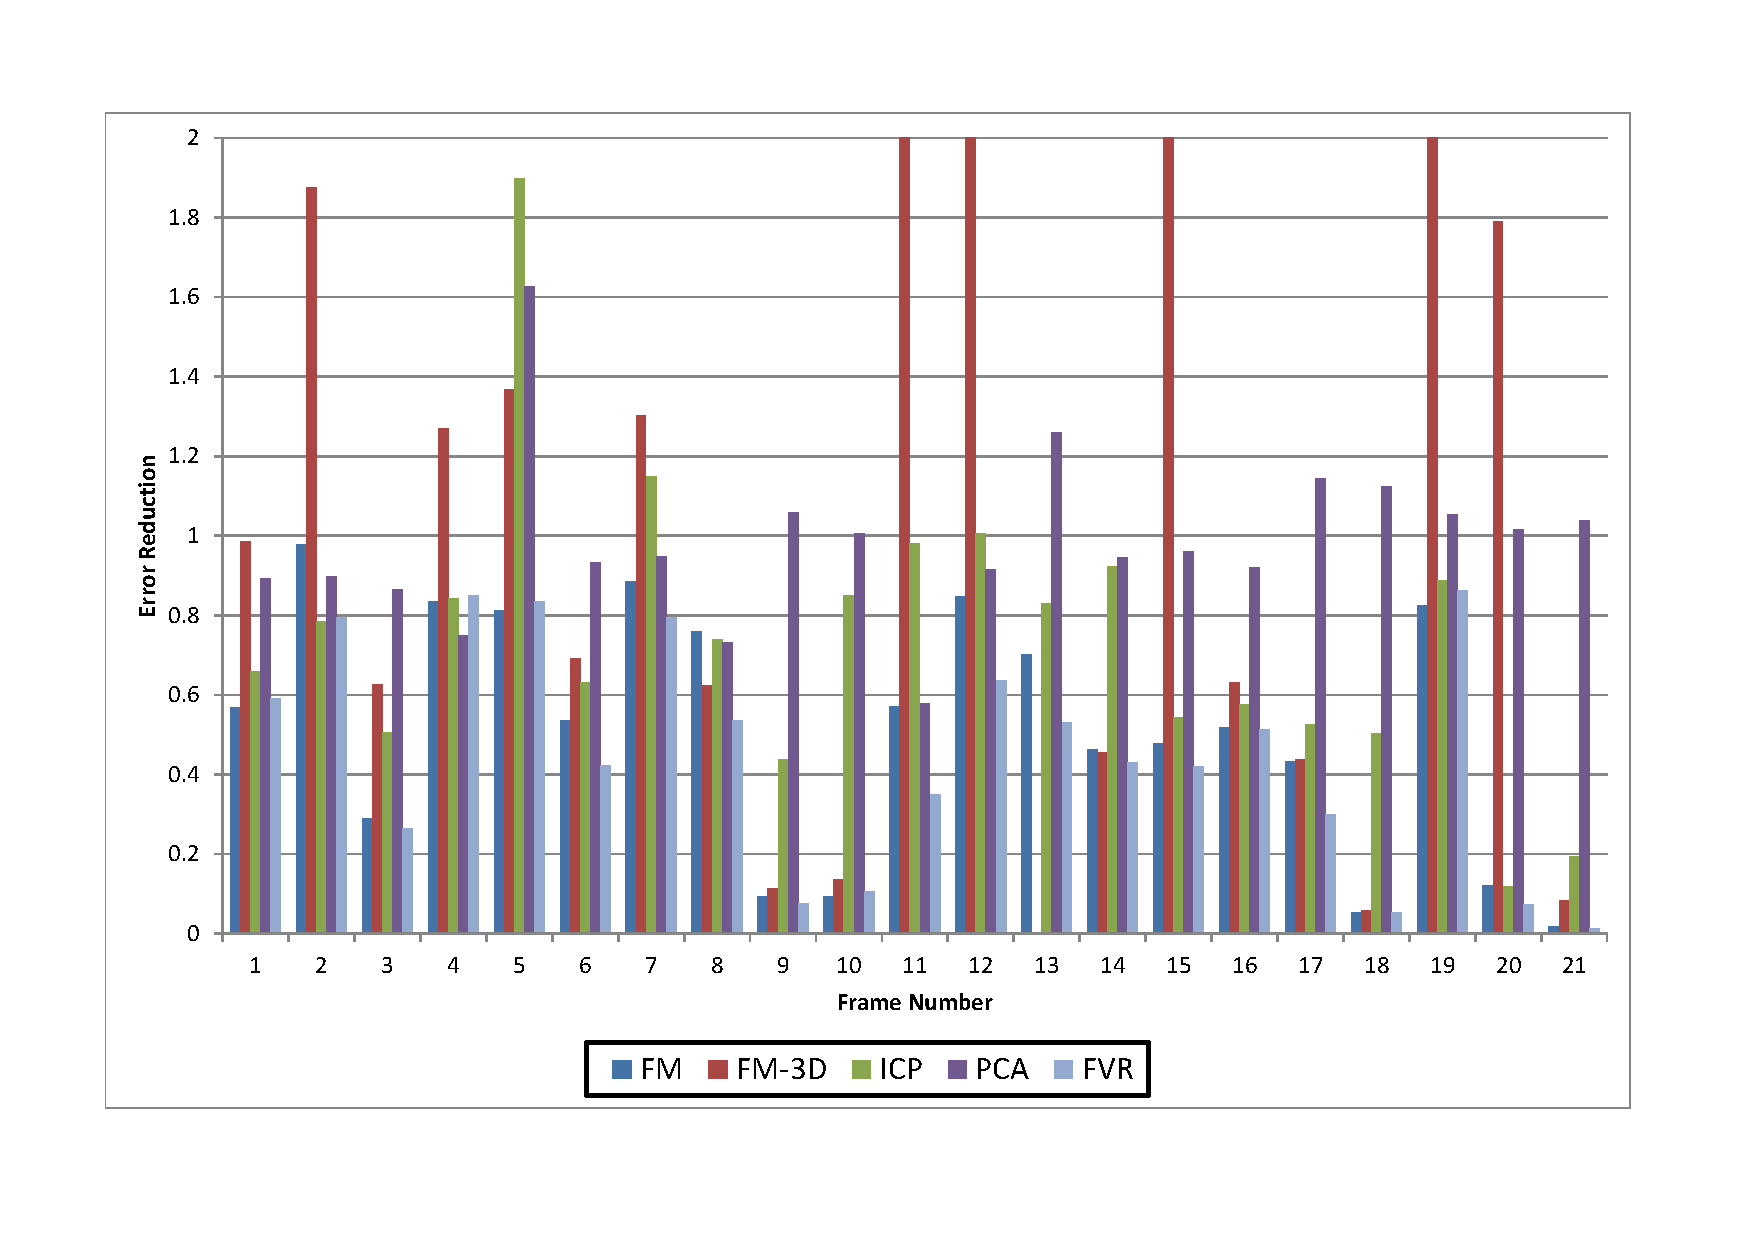
\includegraphics[width=6in]{images/results/Plants_Outdoors_Texture_Confusion_Rotation}
\caption{Registration Error for the Outdoor Plants Texture Confusion Rotation Data Set}
\label{fig:PET17}

\begin{tabular}{ccc}
\hline
\textbf{Algorithm} & \textbf{Average Error $\times$ 1000} & \textbf{\% best result}\\ \hline
FM-2D	& 518.02 & ~23.81\\
FM-3D	& 12791.22 & 0\\
ICP		& 742.37 & ~4.76\\
PCA		& 984.14 & 0\\
FVR		& 450.06 & ~66.67\\
\end{tabular}
\captionof{table}{Statistics for the Outdoor Plants Texture Confusion Rotation Data Set}
%\label{tab:PET17ST}
\end{figure}


The final figure in the pose estimation tests shows another scene taken out-doors. This scene also contains texture confusion, but the camera was rotated about an axis rather than translated in this data-set. Results shown in figure \ref{fig:PET17} indicate that again FVR dominates over the other algorithms, achieving the best result around 67\% of the time and also obtained the lowest average registration error compared to the other algorithms. Surprisingly, it was FM-2D which showed the strongest competition as ICP performed poorly on this data-set especially in comparison to the FVR method. \\


